% !TEX program = xelatex
% basic document config
\documentclass[a4paper,10pt,xetex]{article}
\usepackage[a4paper,top=45mm,right=20mm,bottom=30mm,left=25mm,head=35mm,foot=20mm]{geometry}

% language
\usepackage[german]{babel}

% variable definitions
\providecommand{\documenttitle}{Design}
\providecommand{\documentauthors}{Andreas Saurer \\ Benjamin Schneidinger \\ Josef Erben \\ Raffaele Bof \\ Nicolas Loth}
\providecommand{\documentdate}{25.04.2017}
\providecommand{\documentversion}{1.0.0}

% special commands
\newcommand*{\fullref}[1]{\hyperref[{#1}]{\nameref*{#1} (\ref*{#1})}}
\newcommand{\specialcell}[2][c]{%
  \begin{tabular}[#1]{@{}l@{}}#2\end{tabular}}

% font
% \usepackage{titling}
\usepackage[sfdefault]{roboto}
\usepackage[parfill]{parskip}
\usepackage{soul}

% table
\usepackage{array}
\usepackage{multicol}
\usepackage{longtable,tabu,booktabs}

% links
\usepackage{hyperref}
\hypersetup{
            pdftitle={\documenttitle},
            pdfauthor={\documentauthors},
            colorlinks=true,
            linkcolor=[RGB]{74,144,226},
            citecolor=[RGB]{74,144,226},
            urlcolor=[RGB]{74,144,226},
            breaklinks=true}
\urlstyle{same}  % don't use monospace font for urls

% images
\usepackage{float,graphicx,grffile}
\graphicspath{ {images/} }

\makeatletter
\def\maxwidth{\ifdim\Gin@nat@width>\linewidth\linewidth\else\Gin@nat@width\fi}
\def\maxheight{\ifdim\Gin@nat@height>\textheight\textheight\else\Gin@nat@height\fi}
\makeatother
\setkeys{Gin}{width=\maxwidth,height=\maxheight,keepaspectratio}

\makeatletter
\def\fps@figure{H}
\makeatother

% header and footer
\usepackage{lastpage}
\usepackage{fancyhdr}
\pagestyle{fancy}
\fancyhf{}
\fancyhead[L]{
\includegraphics[height=2cm]{travel-buddy_white}}
\fancyfoot[L]{\fontsize{8}{10}\selectfont\ \documenttitle}
\fancyfoot[R]{\fontsize{8}{10}\selectfont\ Seite\ \thepage\ von\ \pageref*{LastPage}}

\renewcommand{\headrulewidth}{0pt}
\renewcommand{\footrulewidth}{0pt}

% style titles
\usepackage{titlesec}
\titlespacing*{\section}{0pt}{1em}{0pt}
\titlespacing*{\subsection}{0pt}{1em}{0pt}
\titlespacing*{\subsubsection}{0pt}{1em}{0pt}

% configure title page
\title{
  
\includegraphics[width=7cm]{travel-buddy_white}\\[\bigskipamount]
  Design\\[\bigskipamount]
}

\author{\documentauthors}
\date{\parbox{\linewidth}{\centering%
  IT15TA ZH \hspace*{3cm} Gruppe 3\endgraf\bigskip
  Dokumentversion \documentversion, \documentdate\endgraf
}}


\begin{document}

% title page
\maketitle\newpage

% table of contents
{
\hypersetup{linkcolor=black}
\setcounter{tocdepth}{3}
\tableofcontents
}

\newpage

% version log
\section{Versionenlog}\label{versionenlog}

\tabulinesep=1.2mm

\begin{longtabu} to \textwidth { | l | l | X[l] | l | }
  \hline
  \textbf{Version} & \textbf{Datum} & \textbf{Änderung} & \textbf{Author} \\
  \hline
  \endhead

  0.1.0 & 25.04.2017 & Dokument review: Rechtschreib- und Grammatikfehler korrigiert & Beni \\
  \hline

  0.0.10 & 24.04.2017 & Backend Architektur hinzugefügt & Nicolas \\
  \hline

  0.0.9 & 23.04.2017 & Projektmanagement nachgetragen & Raffaele \\
  \hline

  0.0.8 & 23.04.2017 & Interaktionsdiagramm takePhoto() und isNearPoi() erstellen & Josef \\
  \hline

  0.0.7 & 23.04.2017 & GUI Design Mockup hinzugefügt & Andi \\
  \hline

  0.0.6 & 23.04.2017 & Klassenverantwortlichkeiten Frontend ausführen & Josef \\
  \hline

  0.0.5 & 23.04.2017 & Klassendiagramm Frontend erstellt und hinzugefügt & Josef \\
  \hline

  0.0.4 & 23.04.2017 & Interaktionsdiagramme zusammengetragen und hinzugefügt & Andi \\
  \hline

  0.0.3 & 23.04.2017 & Implikationen der Frontend Architektur, Nachtrag Glossar & Josef \\
  \hline

  0.0.2 & 22.04.2017 & Initiale Version der Frontend Architektur & Josef \\
  \hline

  0.0.1 & 21.04.2017 & GUI-Design Text hinzugefügt & Andi\\
  \hline

  0.0.0 & 21.04.2017 & Dokument erstellt & Andi\\
  \hline
\end{longtabu}
\newpage

% start content
\section{Projektmanagement}\label{projektmanagement}
\subsection{Projektstatus}\label{projektstatus}
Das Projekt befindet sich weiterhin auf Kurs. Der nächste Meilenstein wurde ohne
grössere Probleme erreicht. Die folgende Grafik zeigt eine grobe Übersicht
des Projektes, eine detaillierte Übersicht ist unter \fullref{detaillierter-projektplan}
ersichtlich.

\begin{figure}
  \centering
  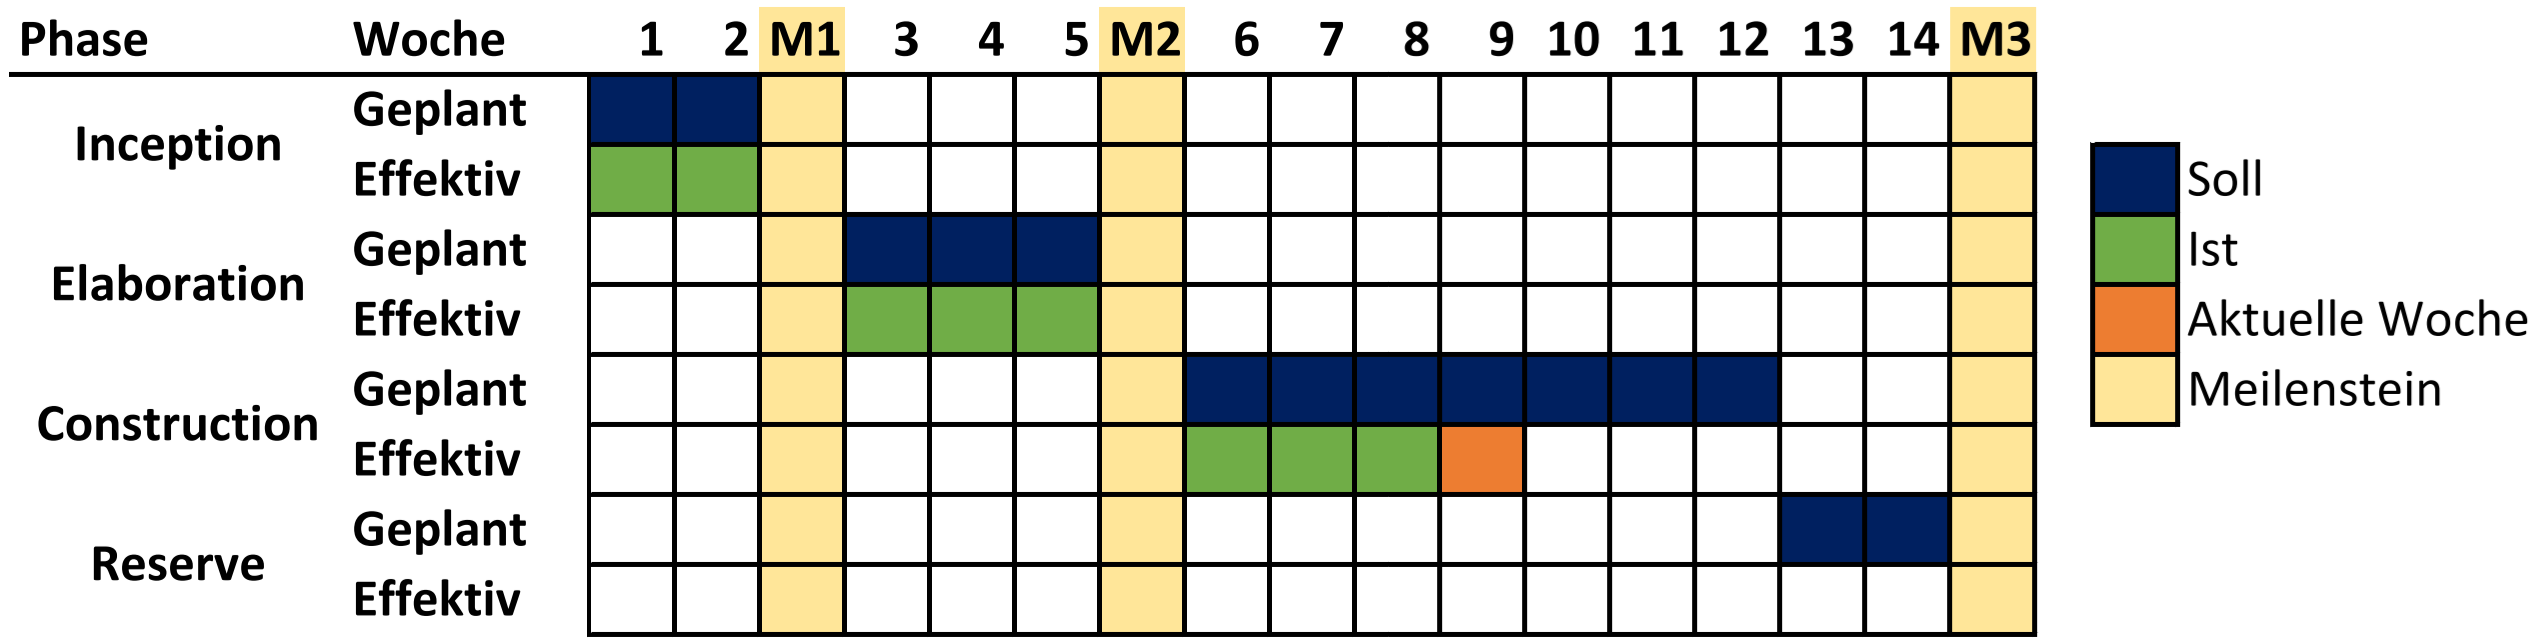
\includegraphics{Grobzeitplan_23.04.2017}
  \caption{Grobzeitplan Stand: 23.04.2017}
\end{figure}


\subsection{Detaillierter Projektplan}\label{detaillierter-projektplan}
\begin{longtabu} to \textwidth { | l | l | X[l] | l | l | }
\hline
\textbf{Phase} & \textbf{Nr.} & \textbf{Arbeitspaket} & \textbf{Soll} & \textbf{Ist} \\\hline
\endhead

\multicolumn{5}{| l |}{ \textbf{Inception} }\\\hline
 & A-01 & Ausgangslage schildern & 5,0 h & 1,0 h \\\hline
 & A-02 & Projektidee beschreiben & 5,0 h & 2,0 h \\\hline
 & A-03 & Kundennutzen analysieren & 5,0 h & 3,0 h \\\hline
 & A-04 & Stand der Technik & 5,0 h & 1,5 h \\\hline
 & A-05 & Konkurenzanalyse & 5,0 h & 3,0 h \\\hline
 & A-06 & Hauptablauf aufzeigen & 5,0 h & 4,0 h \\\hline
 & A-07 & Weitere Anforderungen definieren & 5,0 h & 2,0 h \\\hline
 & A-08 & Ressource beschreiben & 5,0 h & 1,0 h\\\hline
 & A-09 & Projektidee beschreiben & 5,0 h & 6,0 h\\\hline
 & A-10 & Risiken beschreiben & 5,0 h & 0,5h \\\hline
 & A-11 & Grobplanung erstellen & 5,0 h & 3,5 h\\\hline
 & A-12 & Wirtschaftlichkeitsanalyse & 5,0 h & 6,0 h\\\hline
 & A-13 & Projektskizze erstellen (inkl. Präsentation) & 5,0 h & 10,0 h\\\hline
 & A-14 & Entwicklungsumgebung (inkl. Azure, DB) und Projekt aufsetzen für Backend & 10,0 h & 10,0 h\\\hline
 & A-15 & Entwicklungsumgebung und Projekt aufsetzen für Android App & 10,0 h & 11,0 h\\\hline
Total Phase: & 15 & & 85,0 h & 61,0 h\\\hline
\multicolumn{5}{| l |}{ }\\\hline

\multicolumn{5}{| l |}{ \textbf{Elaboration} }\\\hline
 & B-01 & Projekmanagement organisieren & 5,0 h & 6,0 h\\\hline
 & B-02 & Anwendungsfalldiagramm zeichnen & 5,0 h & 0,5 h \\\hline
 & B-03 & Domänenmodell erstellen & 5,0 h & 6,0 h\\\hline
 & B-04 & Architektur beschreiben & 5,0 h & 4,0 h \\\hline
 & B-05 & Zusätzliche Spezifikationen beschreiben & 5,0 h & 7,0 h \\\hline
 & B-06 & System Sequenzdiagramm zeichnen & 5,0 h & 2,5 h \\\hline
 & B-07 & Glossar erstellen & 5,0 h & 0,25 h \\\hline
 & B-08 & Anwendungsfall 1 beschreiben & 1,0 h & 1,0 h \\\hline
 & B-09 & Anwendungsfall 2 beschreiben & 0,5 h & 0,5 h \\\hline
 & B-10 & Anwendungsfall 3 beschreiben & 0,5 h & 0,5 h \\\hline
 & B-11 & Anwendungsfall 4 beschreiben & 0,5 h & 0,5 h \\\hline
 & B-12 & Anwendungsfall 5 beschreiben & 0,5 h & 0,5 h \\\hline
 & B-13 & Anwendungsfall 6 beschreiben & 0,5 h & 0,5 h\\\hline
 & B-14 & Analysedokument erstellen (inkl. Präsentation) & 6,5 h & 15,0 h\\\hline
 & B-15 & Erste Implementierungen an der Web API & 10 h & 20,0 h\\\hline
 & B-16 & Einarbeiten in Android SDK. Erste Implementierung an der Android App & 15 h & 24,0 h\\\hline
Total Phase: & 16 & & 70,0 h & 82,25 h\\\hline
\multicolumn{5}{| l |}{ }\\\hline

\multicolumn{5}{| l |}{ \textbf{Construction} }\\\hline
 & C-01 & Projekmanagement nachtragen & 1,0 h & 1,5 h \\\hline
 & C-02 & UC 1 Liste der verfügbaren Touren & 5,0 h & 6,0 h \\\hline
 & C-03 & UC 1 Starten einer Tour & 6,0 h & 5,5 h \\\hline
 & C-04 & UC 2 Lokalisieren des Benutzers & 6,0 h & 6,0 h \\\hline
 & C-05 & UC 2 Anzeigen des Benutzers auf der Karte & 4,0 h & 4,5 h \\\hline
 & C-06 & UC 3 Foto machen & 4,0 h & \\\hline
 & C-07 & UC 4 Prüfen der Geo koordinaten des Fotos & 6,0 h & \\\hline
 & C-08 & UC 5 Besuchen des nächsten Punktes & 6,0 h & 5,5 h \\\hline
 & C-09 & UC 6 Auslesen der Tourdaten & 5,0 h & \\\hline
 & C-10 & UC 6 Anzeigen der Tourdaten & 4,0 h & \\\hline
 & C-11 & UI gestalten & 8,0 h & \\\hline
 & C-12 & Systemtests durchführen & 12,0 h & \\\hline
 & C-13 & Dokumentation erstellen & 10,0 h & \\\hline
 & C-14 & Benutzeranleitung schreiben & 8,0 h & \\\hline
Total Phase: & 14 & & 85,0 h & \\\hline
\end{longtabu}


\newpage
\subsection{Enteilung Arbeitspakete}\label{enteilung-arbeitspakete}
\begin{longtabu} to \textwidth { | l | l | l | X[l] | }
\hline
\textbf{Wer} & \textbf{Iteration} & \textbf{Paket} & \textbf{Beschreibung} \\\hline
\endhead

Alle                         & 1,2,3,4 & C-01 & Projekmanagement nachtragen \\\hline
Alle                         & 1,2,3,4 & C-11 & UI gestalten \\\hline
Andi, Benjamin, Josef        & 1       & C-02 & UC 1 Liste der verfügbaren Touren \\\hline
Nicolas, Raffaele            & 1       & C-03 & UC 1 Starten einer Tour \\\hline
Andi, Benjamin               & 2       & C-04 & UC 2 Lokalisieren des Benutzers \\\hline
Benjamin, Josef              & 2       & C-05 & UC 2 Anzeigen des Benutzers auf der Karte \\\hline
Raffaele, Andi               & 2       & C-08 & UC 5 Besuchen des nächsten Punktes \\\hline
Benjamin, Josef              & 3       & C-06 & UC 3 Foto machen \\\hline
Josef, Nicolas               & 3       & C-07 & UC 4 Prüfen der Geo-Koordinaten des Fotos \\\hline
Nicolas, Raffaele            & 3       & C-09 & UC 6 Auslesen der Tourdaten \\\hline
Raffaele, Andi               & 3       & C-10 & UC 6 Anzeigen der Tourdaten \\\hline
Josef, Benjamin              & 4       & C-12 & Systemtests durchführen \\\hline
Alle                         & 4       & C-13 & Dokumentation erstellen \\\hline
Andi, Nicolas, Raffaele      & 4       & C-14 & Benutzeranleitung schreiben \\\hline
\end{longtabu}


\subsection{Nächste Iteration}\label{naechste-iteration}
Für die nächste Iteration ist die implementierung der Kartenfunktionen, also die Pakete: \textbf{C-04}, \textbf{C-05}, \textbf{C-08} geplant.
Ziel ist es, bereits einen Teil der Businesslogik umzusetzen und eine minimale Funktionalität für eine erste Demonstration zu erstellen.

\textbf{Backend:} Die App kann die Geo-Koordinaten eines POI einer Tour vom Server anfragen. Die Aufteilung von Front- und Backend bleibt gleich.

\textbf{Frontend (App):} Der Benutzer kann Touren auswählen, sie in einer Vorschau
betrachten und starten.

Die Aufwandsschäztungen der Arbeitspakete sind unter \fullref{detaillierter-projektplan} ersichtlich.

\newpage
\subsection{Risiken}\label{risiken}
\begin{longtabu} to \textwidth { | l | X[l] | l | l | X[l] | }
\hline
\textbf{Nr.} & \textbf{Risiko} & \textbf{Auswirkung} & \textbf{Wahrscheinlichkeit} & \textbf{Massnahmen} \\\hline
\endhead

1 & Schutz der gespeicherten Daten durch unautorisierte Zugriffe & Schwerwiegend & Hoch & Verwendung von Sicherheitsmassnahmen auf dem heutigen Stand der Technik\\\hline
2 & Hohe Kosten für Anwender aufgrund der Verwendung durch Kartenmaterial & Mittel & Hoch & Offlinespeicherung des Kartenmaterials\\\hline
3 & Fehlendes Wissen in der Entwicklung von Mobile Apps & Mittel & Mittel & Aneignen des Wissens mittels Online-Tutorials und Wissensaustausch zwischen Gruppenmitgliedern\\\hline
4 & Höhere Komplexität durch Einbinden von Drittanbieter Software & Gering & Mittel & Auf die Einbindung von Software von Drittanbietern möglichst verzichten\\\hline
5 & Smartphone GPS-Koordinaten ungenau & Gering & Mittel & Die App für Geräte mit zu geringer GPS-Genauigkeit nicht freigeben\\\hline
\st{6} & \st{Keine öffentlichen Karten-API verfügbar} & \st{Schwerwiegend} & \st{Sehr gering} & Entsprechendes Kartenmaterial ist von Google verfügbar\\\hline
\end{longtabu}

\newpage
\section{Frontend Design}\label{design-frontend}
Bei der Architektur und dem Design unterscheiden wir zwischen Backend
(Web Services) und dem Frontend (Android App). Beide Systeme werden parallel und
unabhängig mittels Swagger API Spezifikation entwickelt (siehe \fullref{service-api}).
Durch diesen Swagger Contract als klare Barriere lassen sich Entscheide betreffend
Architektur und Design separat treffen.
Zuerst behandeln wir das Frontend, danach das Backend.
\subsection{Design-Klassendiagramm}\label{design-klassendiagram}
\begin{figure}
  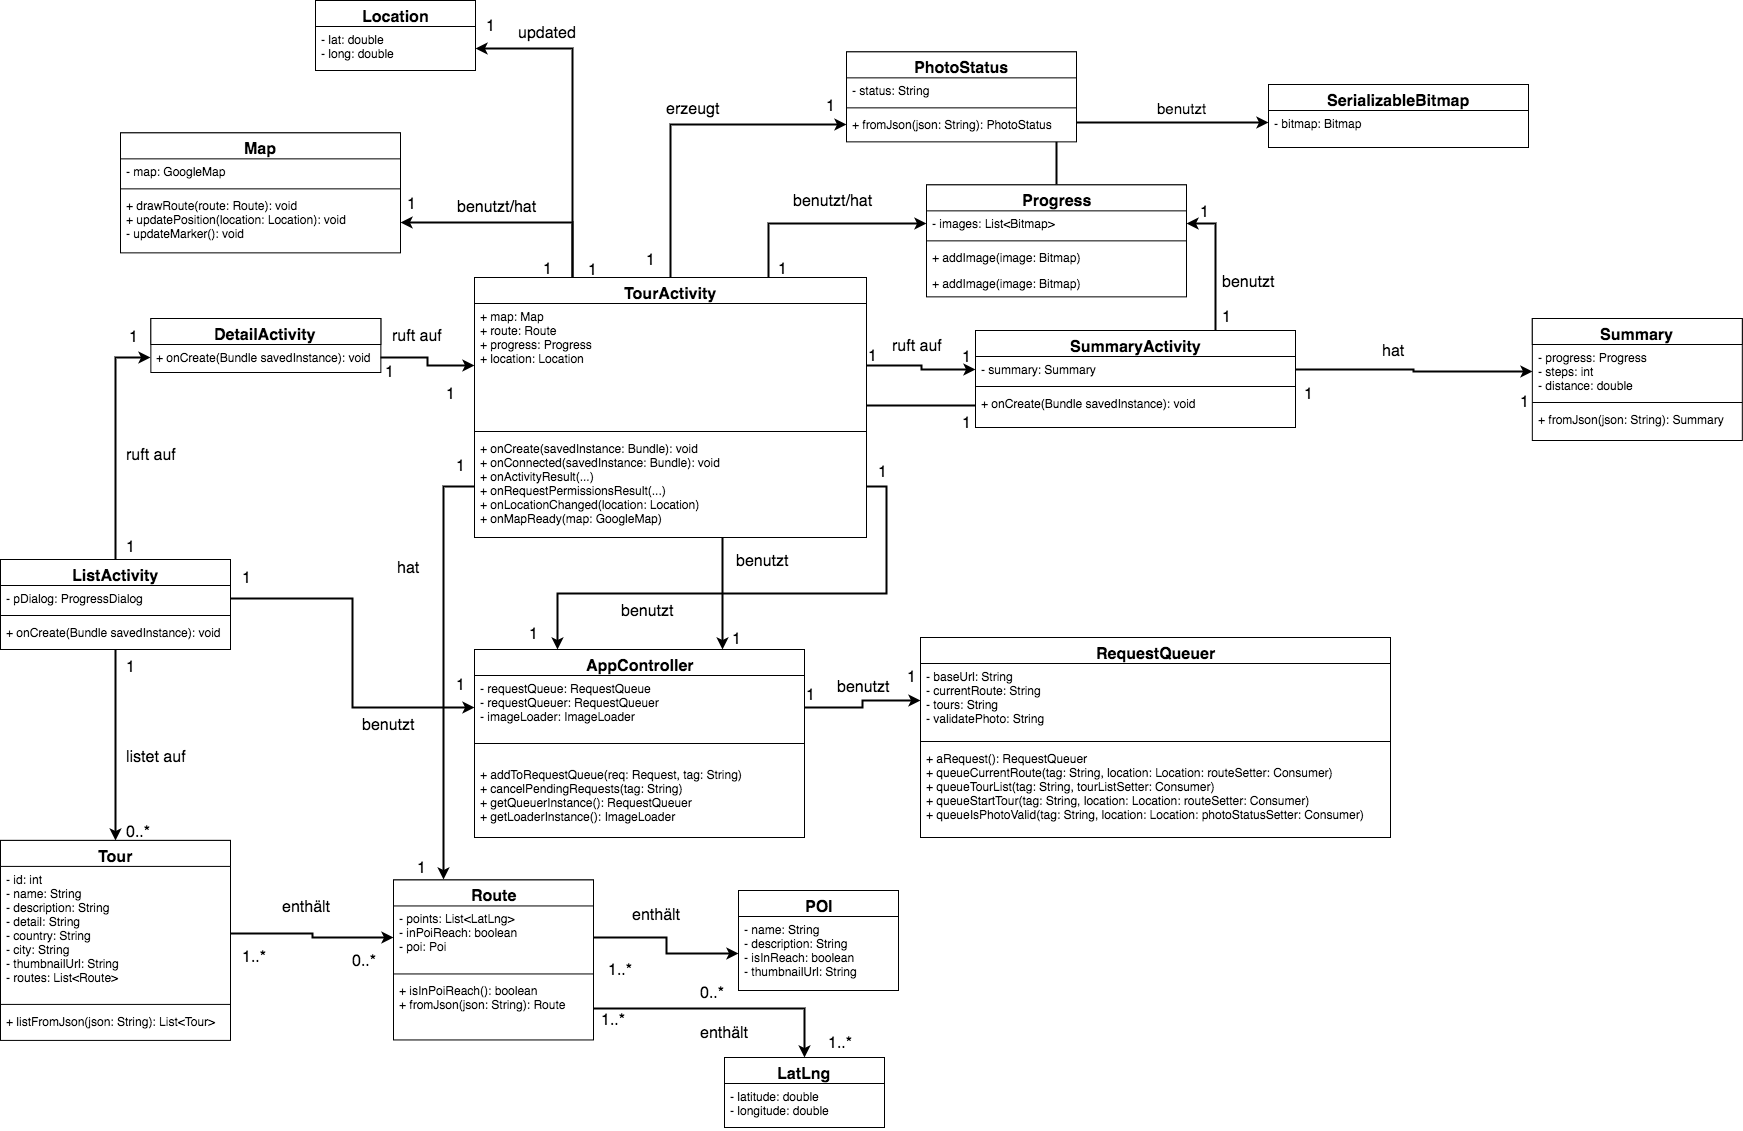
\includegraphics{classdiagram_frontend}
  \caption{Klassendiagramm der App}
\end{figure}

\subsection{Klassenverantwortlichkeiten}\label{klassenverantwortlichkeiten}
In der folgenden Tabelle werden die Klassen mit ihren Hauptverantworlichkeiten
gelistet.

\begin{longtabu} to \textwidth { | l | X[l] |  }
\hline
\textbf{Klasse} & \textbf{Verwantwortlichkeit}\\\hline
\endhead
\textbf{AppController} & Der AppController liefert Instanzen von Singletons.\\\hline
\textbf{RequestQueuer} & Der RequestQueuer wird benutzt, um per HTTP mit dem
Server zu kommunizieren.\\\hline
\textbf{ListActivity} & Die ListActivity zeigt eine Liste von Touren an und
reagiert auf Klick-Events.\\\hline
\textbf{DetailActivity} & Die DetailActivity zeigt eine detaillierte Beschreibung
und ein Thumbnail einer Tour.\\\hline
\textbf{TourActivity} & Die TourActivity speichert die aktuelle Route, aktualisiert
die Position des Nutzers, aktualisiert die Karte und löst HTTP Requests aus.\\\hline
\textbf{SummeryActivity} & Die SummaryActivity erstellt eine \textbf{Summary}
und zeigt diese an.\\\hline
\textbf{Tour} & Die Tour kennt all ihre Routen und dient als Datenklasse. \\\hline
\textbf{Route} & Die Route kennt all ihre Koordinaten und dient als
Datenklasse. \\\hline
\textbf{POI} & Die POI ist eine reine Datenklasse und bildet ein POI ab.\\\hline
\textbf{LatLng} & LatLng ist ein Datentyp, welche eine Position auf dem
Erdball abbildet.\\\hline
\textbf{Map} & Die Map dient als Behählter der Google Map und wird benutzt, um
die Karte zu aktualisieren.\\\hline
\textbf{Location} & Location ist eine Repräsentation eines Ortes und kommt aus
Android SDK.\\\hline
\textbf{PhotoStatus} & PhotoStatus ist eine Datenklasse und repräsentiert das
Ergebnis einer Validierung eines Fotos durch das Backend.\\\hline
\textbf{Progress} & Progress dient als Behälter der während einer Tour geschossenen
Fotos.\\\hline
\textbf{Summary} & Summary wird am Ende einer Tour aus Progress generiert und
bietet dem Nutzer eine Zusammenfassung der Tour.\\\hline
\end{longtabu}

\subsubsection{Klassenverantwortlichkeiten - Knowing and Doing}\label{knowinganddoing-frontend}
Im Folgenden betrachten wie die Knowing- und Doing-Verantwortlichkeiten der Klassen.
\begin{longtabu} to \textwidth { | l | X[2, l] | X[8, l] |  }
\hline
\textbf{Klasse} & \textbf{Knowing} & \textbf{Doing} \\\hline
\endhead
\textbf{AppController} & RequestQueuer & Stellt anderen Objekten den RequestQueuer
als Singleton zur Verfügung.\\\hline
\textbf{RequestQueuer} & keine Abhängigkeiten & Wird in den Activities für asynchrone
HTTP Kommunikation benutzt. Der RequestQueuer baut auch die URLs zusammen und bietet
eine API an, um mit Lambdas Callbacks zu setzen. Dieser ruft die mitgereichten
Consumer mit dem Server Response auf, ohne den Aufrufer zu kennen. Dadurch erreichen
wir lose Kopplung und hohe Wiederverwendbarkeit. \\\hline
\textbf{ListActivity} & AppController, Tour & Die ListActivity gibt über den AppController
einen Callback an den RequestQueuer. Dieser Callback füllt eine Liste von Touren,
welche dem User angezeigt wird. Ein Klick auf eine Tour ruft die DetailActivity auf.
\\\hline
\textbf{DetailActivity} & Tour & Die DetailActivity ist eine einfache Ansicht auf
ein Tour-Objekt und zeigt Details einer Tour an.\\\hline
\textbf{TourActivity} & Map, Route, Progress, Location, AppController & Die TourActivity bildet
unseren Haupt-Use-Case ab: Navigation per Karte durch eine Tour. Die TourActivity
registriert sich selber als Callback beim Google Maps Service und beim Google
Play Location Service. Weiterhin wird das Backend regelmässig nach der aktuellen
Route gefragt. Falls sich der User in der Nähe eines POIs befindet, wird die
Kamera App des Smartphones aktiviert.\\\hline
\textbf{SummeryActivity} & Summary, Progress, RequestQueuer & Die SummaryActivity
bekommt von der TourActivity ein Progress-Objekt. Nach einer Anfrage an das
Backend wird eine \textbf{Summary} Activity erstellt und angezeigt.\\\hline
\textbf{Tour} & Route & Die Tour kennt nur ihre Routen und dient als Datenklasse.
Sie kann sich selber aus JSON instanziieren.\\\hline
\textbf{Route} & LatLng & Die Route kennt all ihre Koordinaten und dient als
Datenklasse. Sie kann sich selber aus JSON instanziieren.\\\hline
\textbf{POI} & keine Abhängigkeiten & Die POI ist eine reine Datenklasse und bildet ein POI ab. Sie
kann sich selber aus JSON instanziieren.\\\hline
\textbf{LatLng} & keine Abhängigkeiten & LatLng ist ein Datentyp, welche eine Position auf dem
Erdball abbildet.\\\hline
\textbf{Map} & GoogleMap & Die Map dient als Behälter der Google Map und wird benutzt, um
die Karte zu aktualisieren. Sie kann den Positionsmarker und die Route zum nächsten
POI zeichnen.\\\hline
\textbf{Location} & keine Abhängigkeiten & kein Verhalten \\\hline
\textbf{PhotoStatus} & keine Abhängigkeiten & kein Verhalten \\\hline
\textbf{Progress} & keine Abhängigkeiten & kein Verhalten \\\hline
\textbf{Summary} & Progress & Summary kann sich selber aus \textbf{Progress}
generieren.\\\hline
\end{longtabu}

Obwohl \textbf{Activities} andere \textbf{Activites} starten können, müssen sie
lediglich deren Klasse kennen. Durch das Messaging System von Android müssen die
Activities keine Instanzen von anderen Activities halten oder diese selber
erzeugen. Im Klassendiagramm (Abbildung 2) sind die Activities zwar miteinander
verbunden, aber durch das Message System (Intents) sind diese lose gekoppelt.


\subsection{Android App Architektur}\label{androidapparchitektur}

Die Architekur der App implementiert eine einfache Version von \textbf{The Clean Architecture} \cite{TCA}.
Im nachfolgenden Abschnitt werden einige wichtige Punkte von \textbf{The Clean Architecture}
erläutert, um die Implementation in TravelBuddy aufzuzeigen. Eine umfassende
Einleitung findet man bei Robert Martin (Uncle Bob) \cite{CC}.
\begin{figure}
  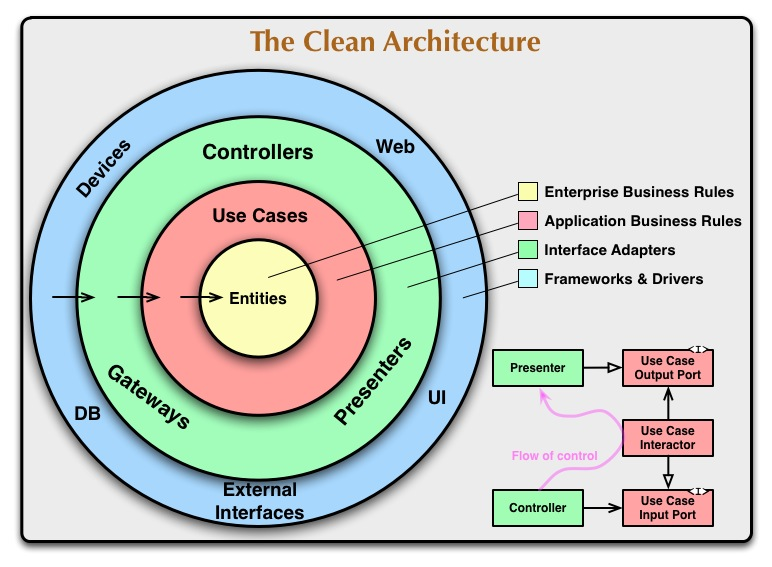
\includegraphics{cleanarchitecture}
  \caption{Schema von The Clean Architecture}
\end{figure}

\subsubsection{Abhängigkeiten - Dependency Rule}\label{dependencyrule}
Diese einfache Regel stellt lose Kopplung und gute Testbarkeit sicher.
Die \textbf{Dependency Rule} besagt, dass die Source Code Abhängigkeit nach innen zeigt.
Das heisst, dass eine bestimmte Schicht niemals die äussere Schicht kennt.
Man hat beispielsweise einen HTTP Client (Web) in der äussersten Schicht und
einen Parser (Gateway) in der direkt darunterliegenden Schicht. Nach der
\textbf{Dependency Rule} darf es keine Referenzen im Parser zum HTTP-Client geben.

\subsubsection{Bedeutung der Schichten}\label{layers}
\begin{longtabu} to \textwidth { | l | X[l] |  }
\hline
\textbf{Bezeichnung der Schicht} & \textbf{Bedeutung und Beispiele}\\\hline
\endhead
\textbf{Frameworks and Drivers} & Die äusserste Schicht \textbf{Frameworks and Drivers}
ist für die Kommunikation mit der äusseren Welt zuständig. Dazu zählen zum
Beispiel Kommunikation mit dem User per UI, Persistierung von Daten in Datenbanken
oder Kommunikation mit externen Services per HTTP. Die äusserste Schicht beinhaltet
aber auch Frameworks.\\\hline
\textbf{Interface Adapters} & Die nachfolgende Schicht heisst \textbf{Interface Adapters}.
Diese Schicht hat zur Aufgabe, die Daten in eine für die Use-Cases- und Entities-Schicht
möglichst angenehme Form zu bringen.\\\hline
\textbf{Use Case} & Die zweitinnerste Schicht nennt man \textbf{Use Case} Layer.
Hier werden die applikationsspezifischen Businessregeln, also die Use Cases abgebildet.
Die eigentliche Businesslogik existiert also in dieser Schicht. Zu beachten ist aber,
dass es hier nur um Verhalten und nicht um Daten geht.\\\hline
\textbf{Entities} & Die eigentlichen Businessobjekte gehören in die innerste
Schicht, genannt \textbf{Entities}. Diese Schicht hat keine Abhängigkeiten zu
anderen Schichten und beinhaltet die generellen Regeln der Domäne. Bei Änderungen
in äusseren Schichten sind mit hoher Wahrscheinlichkeit keine Änderungen in dieser
Schicht notwendig. Zur Abgrenzung zur oberen Schicht \textbf{Use Case}: Die Schicht \textbf{Entities}
muss nicht angepasst werden, falls sich Use Cases ändern. Dies ist der Fall, da
sich die allgemeinen Domänenregeln in der Regel nicht ändern.\\\hline
\end{longtabu}

\subsubsection{The Clean Architecture bei TravelBuddy}
Die TravelBuddy App ist ein Spezialfall einer Android App. Da das Team das grösste
Risiko bei der Android-Entwicklung sah, wurde entschlossen, in der App selber so
wenig Businesslogik wie möglich auszuführen.
Dies hat natürlich einen Einfluss auf die Architektur, wie im folgenden Abschnitt aufgezeigt wird.

\begin{longtabu} to \textwidth { | l | X[l] |  }
\hline
\textbf{Schicht} &  \textbf{Zuständigkeiten und Beispiele} \\\hline
\endhead
\textbf{Frameworks and Drivers} & Kümmert sich um Lifecycle der App, die Berechtigungen
und um die Einbettung ins Android Betriebssystem, setzt HTTP Requests ab und reicht
HTTP Responses weiter, aktualisiert Standortdaten, bekommt Bilder von der
Smartphone-Kamera, erhält Karte von der Google Maps App\\\hline
\textbf{Interface Adapters} & Parst Antworten des Servers in String-Form und wandelt
diese Datenobjekte um, transformiert Kartendaten und Standortdaten in für die App
einfach zu handhabbare Form\\\hline
\textbf{Use Case} & Hier kommt der einfache Fall der Android App zugute: Die App
enthält sehr wenig Businesslogik. Die Use Cases sind im Backend implementiert.\\\hline
\textbf{Entities} & Enthält die Datenobjekte, welche die Domänenregeln abbilden:
Eine Tour besteht aus einer Liste von Routen, jede Route hat ein POI zum Ziel\\\hline
\end{longtabu}

\subsubsection{Implikationen}\label{implications}
Die Anwendung der \textbf{Clean Architecture} bringt natürlich sowohl Vor- als
auch Nachteile. Die nachfolgende Liste zeigt Implikationen und Auswirkungen der
gewählten Architektur auf das Design und die Umsetzung der App.
\begin{enumerate}
  \item \textbf{Klare Abhängigkeiten:} Durch die klar definierten Abhängikeiten
    lassen sich Kosten und Aufwände von Änderungen/Erweiterungen besser abschätzen:
    Wollen wir beispielsweise die Technologie zur Kommunikation mit dem
    Backend von REST/HTTP auf WebSockets/PubSub ändern, wissen wir, dass sich
    die inneren beiden Schichten nicht ändern. Wir müssen lediglich die äussere
    Schicht anpassen, damit sie WebSockets handhabt. Der Parser, in der direkt
    darunterliegenden Schicht, erhält idealerweise den gleichen Response Body
    und muss nicht angepasst werden.
  \item \textbf{Gute Testbarkeit:} Die Businesslogik ist vollkommen unabhängig
    von verwendeteten Frameworks und der UI. Diese kann ohne eine laufende
    Android Instanz getestet werden. Das führt zu kürzeren Feedback Loops
    bei der Ausführung von Unit Tests und dadurch zur effizienteren Entwicklung
    (ein komplettes Re-deployment entfällt).
    Da in den beiden inneren Schichten keine Abhängigkeit zu externen Systemen
    besteht, lassen sich diese ohne grossen Aufwand (z.B. Testing-Setup) testen.
  \item \textbf{Keine Abhängikeit zum Betriebssytem:} Aus Punkt 1 und 2
    leitet sich dieser Punkt ab: Alle Abhängigkeiten befinden sich um
    äussersten Layer. Falls die App auch auf anderen Systemen lauffähig sein soll, dann muss im Idealfall nur eine Schicht angepasst werden. Durch Projekte wie RoboVM \cite{RV} und Intel Multi OS Engine \cite{MOE} können wir den bestehenden Java Code
    sogar auf iOS Geräten laufen lassen. Unsere App ist damit sogar nur lose
    zum Betriebssystem gekoppelt.
  \item \textbf{Overhead:} Da die App in der ersten Version praktisch keine
    Businesslogik enthalten wird, entfällt die \textbf{Use Case} Schicht.
    Dadurch bleiben eigentlich die anderen drei Layer, die mit der ersten
    Version ebenfalls noch überschaubar ausfallen. Man könnte argumentieren,
    dass diese Architektur etwas zu hoch gegriffen ist für die Anforderungen
    des Prototypen. Im Gegensatz zu Design lässt sich Architektur nicht oder
    sehr schwer inkrementell entwickeln. Wir denken, dass der Aufwand für Änderungen
    der Architektur im späteren Verlauf (etwa durch neue Anforderungen) den
    initialen Mehraufwand rechtfertigt.
\end{enumerate}

Durch die gewählte Architektur erreichen wir gute Testbarkeit mit klaren
Abhängigkeiten. Der Mehraufwand wird dadurch gerechtfertigt, dass Änderungen
von Technologien nur kleine, kalkulierbare Anpassungen zur Folge haben.

\subsubsection{Activities}\label{activities}
Die App selber besteht aus drei Haupt-Activities. \textbf{Activities} ist ein
Konzept von Android, sie bilden eine User-Ansicht ab und bilden des Skelett
der App. Abbildung 4 veranschaulicht alle möglichen Zustände und deren
Änderungen.
\begin{figure}
  \centering
  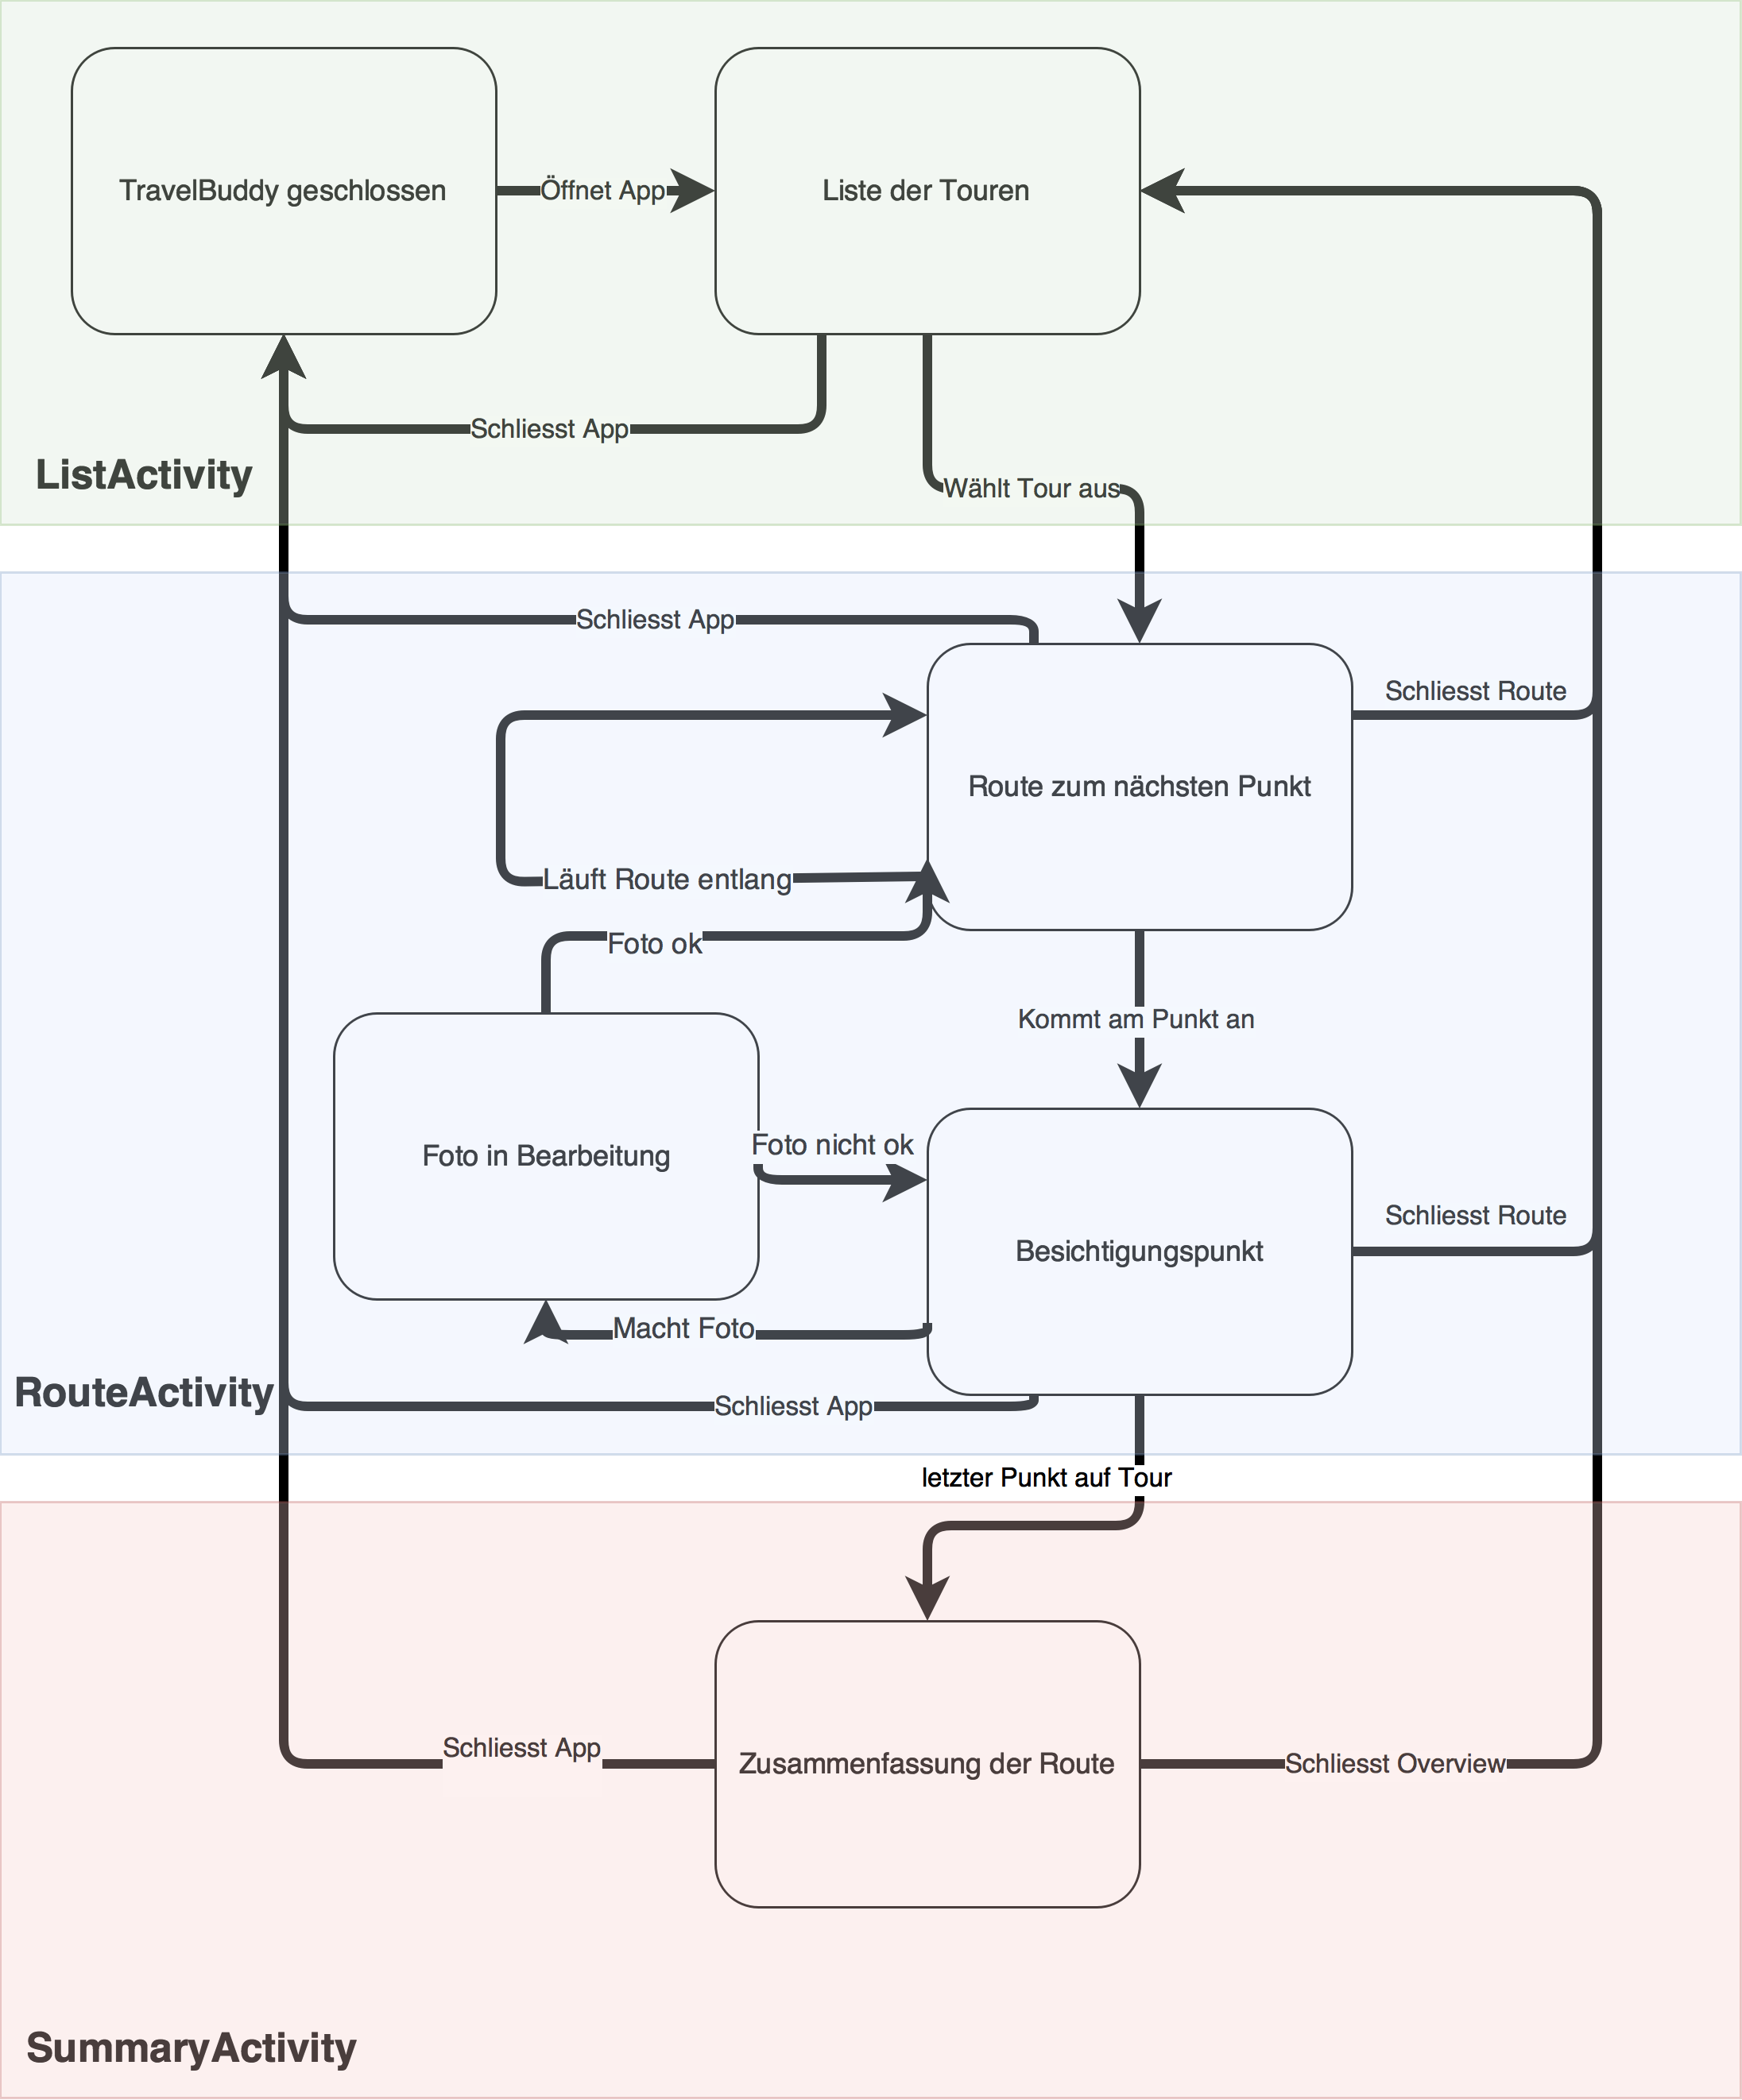
\includegraphics{state-diagram}
  \caption{Zustandsänderungsdiagramm}
\end{figure}


\section{Backend Design}\label{backend-design}
\subsection{Service API}\label{service-api}
Die API ist als Webservice aufgebaut welcher funktionale Requests beantworten kann. Es wird kein direkter Datenzugriff
\"uber CRUD Methoden zur Verf\"ugung gestellt. Die Business-Logik wird wenn m\"oglich vollst\"andig im Service
abgehandelt. So ist die Funktionalit\"at des ganzen Systems gekapselt und unabh\"angig von allenfalls in der Zukunft
weiteren entwickelten Clients.

Nachfolgend sind alle geplanten Service Methoden nach Controller gruppiert aufgelistet. Eine
interaktive Version ist unter \fullref{swagger} verlinkt.

\begin{figure}
  \centering
  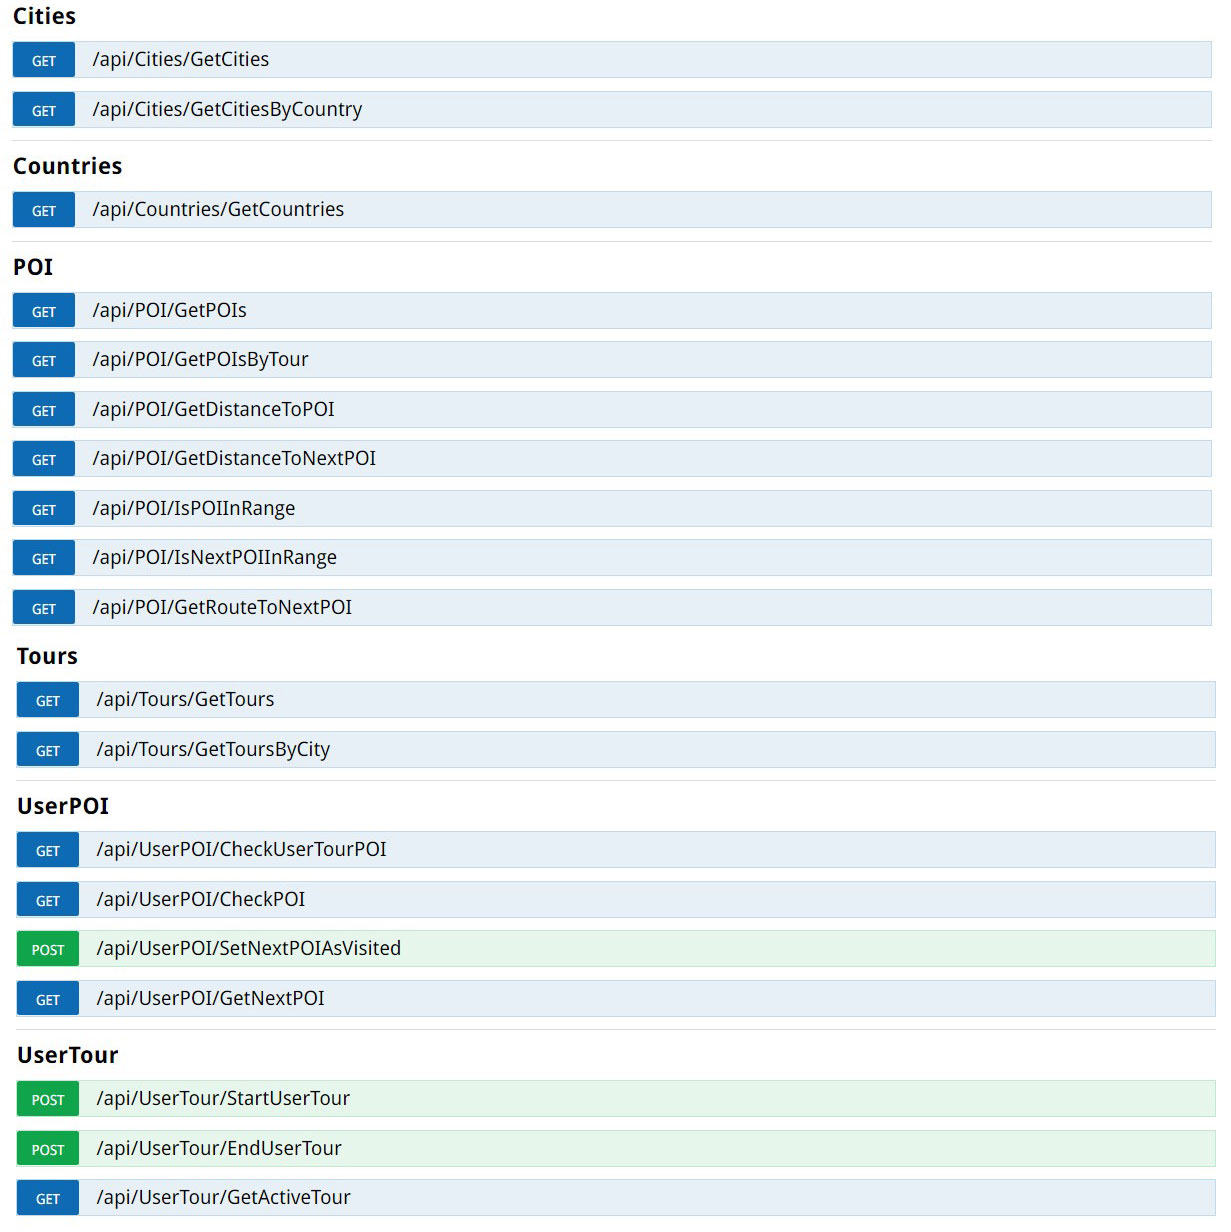
\includegraphics{swagger}
  \caption{Übersicht API}
\end{figure}

Controller:

\begin{longtabu} to \textwidth { | l | X[l] | }
\hline
\textbf{Controller} & \textbf{Beschreibung} \\
\hline
\endhead

Cities & Implementiert alle Funktionalit\"aten zum Abfragen und \"Andern von
  St\"adte-Daten\\ \hline
Countries & Implementiert alle Funktionalit\"aten zum Abfragen und \"Andern von
  L\"ander-Daten\\ \hline
POI & Implementiert alle Funktionalit\"aten zum Abfragen und \"Andern von Point of
Interests, welche durch eine Tour verkn\"upft sind.\\\hline
Tours & Implementiert alle Funktionalit\"aten zum Abfragen und \"Andern von Touren.\\\hline
UserPOI & Implementiert alle Funktionalit\"aten zum Abfragen und \"Andern von UserPOIs.
  Ein User POI ist ein Point of Interest welcher von einem Benutzer besucht wurde oder
  welcher ein Benutzer im Rahmen seiner gestarteten Tour als n\"achstes besuchen muss.\\\hline
UserTour & Implementiert alle Funktionalit\"aten zum Abfragen und \"Andern von UserTouren.
  Eine UserTour ist eine Tour die von einem Benutzer gestartet wurde.\\\hline
\end{longtabu}

Methoden:

\begin{longtabu} to \textwidth { | l | X[l] | }
\hline
\textbf{Methode} & \textbf{Beschreibung} \\
\hline
\endhead

api/Cities/GetCities &
Liefert eine Liste aller vorhandenen St\"adte.\\\hline
api/Cities/GetCitiesByCountry &
Liefert eine Liste aller vorhandenen St\"adte in einem bestimmten Land.\\\hline
  api/Countries/GetCountries &
Liefert eine Liste aller vorhandenen L\"ander.\\\hline
api/POI/GetPOIs &
Liefert eine Liste aller vorhandenen POIs.\\\hline
api/POI/GetPOIsByTour &
Liefert eine Liste aller POIs zu einer bestimmten Tour.\\\hline
api/POI/GetDistanceToPOI &
Gibt aufgrund von Geokoordinaten die Distanz bis zu einem bestimmten POI zur\"uck.\\\hline
api/POI/GetDistanceToNextPOI &
Gibt aufgrund von Geokoordinaten und einer Benutzer-ID die Distanz bis zu einem n\"achsten POI
  den der Benutzer mit seiner gestarteten Tour besuchen muss.\\\hline
api/POI/IsPOIInRange &
Gibt aufgrund von Geokoordinaten zur\"uck, ob diese gen\"ugend nahe an einem POI sind. Die
  erlaubte Distanz kann als optionaler Parameter mitgegeben werden. \\\hline
api/POI/IsNextPOIInRange &
Gibt aufgrund von Geokoordinaten und einer Benutzer-ID zur\"uck, ob die Koordinaten gen\"ugend
  nahe am n\"achsten POI, den der Benutzer mit seiner gestarteten Tour besuchen muss, ist.

Die erlaubte Distanz kann als optionaler Parameter mitgegeben werden.\\\hline
api/POI/GetRouteToNextPOI &
Liefert aufgrund einer Benutzer-ID die Route als einzelne Navigationspunkte zum n\"achsten
  POI, den der Benutzer mit seiner gestarteten Tour besuchen muss.\\\hline
api/Tours/GetTours &
Gibt alle vorhandenen Touren zur\"uck.\\\hline
api/Tours/GetToursByCity &
Gibt alle vorhanden Touren in einer bestimmten Stadt zur\"uck.\\\hline
api/UserPOI/CheckUserTourPOI &
Markiert einen bestimmten POI in einer UserTour als besucht.\\\hline
api/UserPOI/CheckPOI &
  Markiert einen bestimmten POI f\"ur eine angegebene Tour und eine definierte Benutzer-ID als
  besucht.\\\hline
api/UserPOI/SetNextPOIAsVisited &
Markiert den n\"achsten POI, den ein bestimmter Benutzer aufgrund seiner aktiv gestarteten
  Tour besuchen muss, als besucht.\\\hline
  api/UserPOI/GetNextPOI &
Liefert f\"ur eine Benutzer-ID den n\"achsten POI zur\"uck, den der Benutzer besuchen
  muss.\\\hline
api/UserTour/StartUserTour &
Startet eine definierte Tour f\"ur einen bestimmten Benutzer. Liefert direkt eine Auflistung
  aller POIs und Routenpunkte dieser Tour zur\"uck.\\\hline
api/UserTour/EndUserTour &
Beendet die aktive UserTour f\"ur einen bestimmten Benutzer. \\\hline
api/UserTour/GetActiveTour &
Gibt die aktive Tour des Benutzers zur\"uck.\\\hline
\end{longtabu}

\subsubsection{Versionierung der API}\label{versionierung-api}
F\"ur gr\"ossere \"Anderungen an der API soll aus Kompatibilit\"atsgr\"unden eine neue Version erstellt und parallel zu
\"alteren Versionen deployt werden. Swashbuckle bietet auch hierf\"ur die notwendige Funktionalit\"at zur Versionierung
an.

\subsection{Externe Frameworks}\label{externe-frameworks}
Zur Implementierung von architektonischen und business-funktionalen Anforderungen, die nicht bereits mit ASP.NET MVC und
Web API abgedeckt sind, sollen bereits bestehende Libraries und Frameworks verwendet werden. Die nachfolgende Tabelle
listet die zu verwenden Frameworks auf:

\begin{longtabu} to \textwidth { | l | l | l | X[l] | }
\hline
\textbf{Framework} & \textbf{Version}  & \textbf{Typ} & \textbf{Beschreibung} \\
\hline
\endhead

Google Maps API &
0.65 &
Funktional &
Wird verwendet um die funktionalen Anforderungen wie Routenberechnung usw. zu
  implementieren.\\\hline
Ninject &
3.2.0 &
Architektur &
Ninject ist ein Dependency Injection Framework, welches eine Integration f\"ur ASP.NET
  anbietet. Mit Dependency Injection sollen die einzelnen Repositories den Controllern zur Verf\"ugung gestellt werden.
  Dadurch soll ebenfalls gew\"ahrleistet werden, dass pro Request und Repository nur genau eine Datenbankverbindung
  aufgebaut und dann auch wieder sauber geschlossen wird. So werden Performance- und Datenkonsistenzprobleme, sowie
  Probleme mit nicht geschlossenen Datenbankverbindungen vermieden.\\\hline
Swashbuckle &
5.2.1 &
Architektur &
Swashbuckle erm\"oglicht das automatische Generieren und Anzeigen von Swagger Interface
  Descriptions zur Laufzeit. Mit Hilfe dieser Descriptions k\"onnen die Services einfacher integriert werden, indem zum
  Beispiel die Datenobjekte oder Proxy-Klassen auf Konsumentenseite automatisch generiert werden k\"onnen.\\\hline
Log4Net &
2.0.8 &
Nicht-Funktional &
Framework zum Loggen von Fehlern, Warnungen und Debug-Informationen an verschiedene
  Appenders wie Datenbank oder Logfile.\\\hline
\end{longtabu}


\subsection{Architektur}\label{backendarchitektur}
Das nachfolgende Diagramm zeigt die Detail-Architektur des Backends. Weitere grundlegende
Informationen zum eingesetzten Technologie-Stack befinden sich im Dokument Anforderungsanalyse.

\begin{figure}
  \centering
  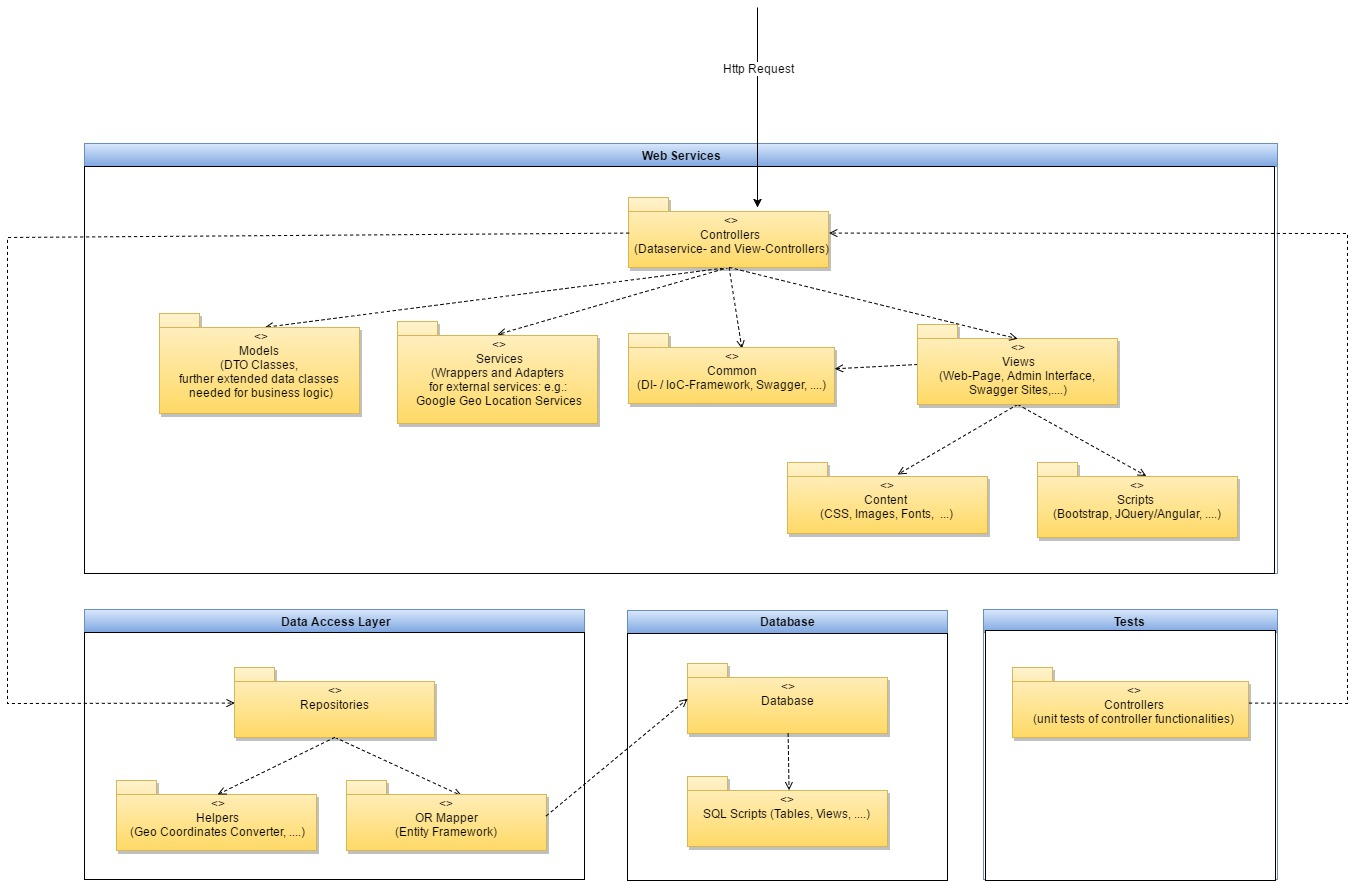
\includegraphics{backend_architektur}
  \caption{Backend Architektur}
\end{figure}

\begin{longtabu} to \textwidth { | l | l | X[l] | }
\hline
\textbf{Layer} & \textbf{Package}  & \textbf{Beschreibung} \\
\hline
\endhead

Web Services &
Controllers &
Controllers beinhaltet alle WebAPI- sowie MVC-Controller, welche die ankommenden Requests
  bearbeiten.

Ein Controller hat mindestens eine Methode und wird \"uber eine spezifische Sub-Url
  aufgerufen. ASP.NET WebAPI/MVC \"ubernimmt das automatische Mapping des ankommenden Requests mit den entsprechenden
  Parametern inkl. Request-Type \ und findet die passende Methode des Controllers, die diesen Request verarbeiten kann.
  Ein API Controller liefert nur Daten in JSON oder XML Format und keine darstellungsspezifischen Informationen.

Zu einem sp\"ateren Zeitpunkt k\"onnen f\"ur die Implementierung der Web-Applikation als
  Administrations-Interface MVC-Controller erstellt werden welche eine entsprechende HTML View zur\"uckgeben. S\"amtliche
  Daten sollen aber auch hier dynamisch \"uber API-Controller mit AJAX-Requests geladen werden. Es sollen keine Seiten
  mit Daten serverseitig gerendert werden.\\\hline
Web Services &
Models &
Dieses Paket beinhaltet alle Model-Klassen welche in den Webservices ben\"otigt werden. Diese
  Klassen unterscheiden sich durch Attribut-Erg\"anzungen (z.B. f\"ur aggregierte oder aufgeschl\"usselte Datenfelder)
  gegen\"uber den vom Entity-Framework generierten Datenklassen welche prim\"ar die Datenbankstruktur abbilden.

Hier befindet sich auch die Funktionalit\"at zum Mappen der Entity-Framework-Datenklassen auf
  DTO Klassen.\\\hline
Web Services &
Services &
Hier sind alle Adapter- und Wrapperklassen f\"ur externe Service angesiedelt, welche f\"ur
  weitere Funktionalit\"aten vom Backend aufgerufen werden.\\\hline
Web Services &
Common &
Dies beinhaltet alle Klassen und Funktionalit\"aten welche \"uber das ganze Projekt hinweg
  ben\"otigt werden. Hierbei handelt es sich zum Beispiel um die ganze Dependency Injection oder Swagger
  Funktionalit\"at.\\\hline
Web Services &
Views &
Zu einem sp\"ateren Zeitpunkt soll neben den Datenservices auch eine Webapplikation erstellt
  werden, welche das Administrieren der Daten erm\"oglichen soll. Hierf\"ur k\"onnen in diesem Package HTML Views
  erstellt werden.\\\hline
Web Services &
Content &
Content beinhaltet den Content der f\"ur die Darstellung der Views ben\"otigt wird wie zum
  Beispiel CSS-Files, Bilder, Fonts usw.\\\hline
Web Services &
Scripts &
Hier werden alle Skripts abgelegt die client-seitig ben\"otigt werden. Es handelt sich hierbei
  vor allem um selbst erstellte Javascript-Funktionalit\"aten und Javascript Frameworks wie JQuery, Angular, Bootstrap
  usw. Die Details zur Implementierung des Webinterfaces werden zu einem sp\"ateren Zeitpunkt genauer definiert.\\\hline
Data Access Layer &
Repositories &
Grunds\"atzlich existiert f\"ur jede Datenklasse aus der Datenbank ein Repository, welche die
  Daten (teil-)aggregiert und funktional zur Verf\"ugung stellt. Dadurch ist die Wiederverwendbarkeit grundlegender oder
  kombinierter Datenabfragen gew\"ahrleistet.\\\hline
Data Access Layer &
Helpers &
Zum Beispiel f\"ur das Umwandeln der Koordinaten-Angaben vom MSSQL-Format in einzelne
  Werteangaben f\"ur L\"angen- und Breitengrade werden Helferklassen ben\"otigt, welche hier angesiedelt sind.\\\hline
Data Access Layer &
OR Mapper &
Als klassischer OR Mapper wird das Entity Framework mit dem Database First Vorgehen verwendet.
  Dies bedeutet, dass basierend auf der Datenbank automatisch Proxy-Datenklassen vom Entity-Framework generiert
  werden.\\\hline
Database &
Database &
Das Datenbankprojekt wird vollst\"andig als MSSQL Datenbank Projekt umgesetzt. Damit werden
  automatisch \"Anderungen an den SQL Dateien im Projekt getrackt und es k\"onnen unter Beachtung dieser \"Anderungen
  automatisch Datenbank Installations-Packages (DACPAC) generiert werden, welche den initialen Stand oder ein Delta
  beinhalten.\\\hline
Database &
SQL Scripts &
Die eigentlichen SQL Skripts f\"ur Tables, Views oder weitere Datenbank-Elemente.\\\hline
Tests &
Controllers &
Dieses Testprojekt implementiert alle Unit-Tests zum automatischen Testen der WebAPI
  Controller-Funktionalit\"aten. \\\hline
\end{longtabu}

\subsubsection{Ablauf eines Request und Datenfluss aus technischer Sicht}\label{ablauf-request}
Der nachfolgende Prozess zeigt den programmatischen Standardablauf eines Request im Backend, inklusive dem Datenfluss
von der Datenbank bis zum Inhalt in der HTTP-Response, auf:

\begin{enumerate}
  \item
    Der Controller erh\"alt einen Request. Bei der Instanzierung des Controller werden automatisch \"uber Dependency Injection
    die ben\"otigten Repositories instanziert und mitgegeben. Ein Repository erstellt bei der Instanzierung automatisch
    eine Datenbankverbindung. F\"ur einen Request wird so pro Repository nur eine einzige Datenbankverbindung aufgebaut, da
    auch nur eine Repository-Instanz erstellt wird.
  \item
    Die Repository-Klasse extrahiert die ben\"otigten Daten mit LINQ-Queries und gibt diese immer als IQueryable
    R\"uckgabewert zur\"uck. Damit lassen sich einzelne Repository-Abfragen theoretisch auch hintereinanderschalten oder es
    sind weitere Operationen auf dem Datensatz m\"oglich.
  \item
    Die Daten werden \"uber das Datenmodel vom Entity-Framework beim Materialisieren des LINQ-Queries geladen.
  \item
    Die Controller-Funktion erstellt eine Instanz des DTO. Dies geschieht entweder mit automatischen Mapping \"uber
    Reflection f\"ur gleiche Felder wie die Datenklassen des Entity Framework Modells oder falls ben\"otigt mit manuellen
    Mapping \"uber eine wiederverwendbare Lambda Function Expression f\"ur einzelne oder mehrere Properties. Diese kann
    direkt auf das erhaltene IQueryable als Select-Befehl angewendet werden.
  \item
    Der Controller gibt das Resultat zusammen mit einem Statuscode zur\"uck.
  \item
    Die Repository Instanz wird nicht mehr ben\"otigt. Die Datenbankverbindung wird geschlossen und die Instanz disposed.
\end{enumerate}

\subsubsection{Dependency Injection}\label{dependency-injection}
Als Dependency Injection Framework f\"ur die Umsetzung des Inversion of Control Patterns wird Ninject eingesetzt.
Ninject bietet eine statische Konfiguration zum Binden von Interfaces an bestimmte Klassen welche bei einer solchen
Anfrage instanziert werden m\"ussen. Eine solche Implementierung bietet eine bessere Performance als wenn die zu
instanziierenden Klassen im ganzen Projekt zuerst gesucht werden m\"ussen. Die Services welche injected werden, sollen
als One-Per-Request Modul definiert sein.


Da ein Controller von der erfolgreichen Instanzierung seines ben\"otigten Repositories abh\"angig ist (strong-coupled),
w\"are in einer n\"achsten Version eine Implementierung der Repositories als Lazy-Object sinnvoll. Dadurch w\"urde die
Instanzierung erst beim ersten Zugriff innerhalb des Controllers geschehen und es k\"onnte bei einem Problem spezifisch
darauf reagiert werden. Bei der direkten Injection ist dies nur begrenzt m\"oglich, da dann entweder vorher einen Fehler
geworfen wird oder aber die injezierten Parameter als Null daherkommen.

\subsubsection{Logging}\label{logging}
Das Logging wird mit Hilfe der Log4Net Library implementiert. Geloggt werden soll in t\"agliche Rolling-Logfiles, was
als Appender in Log4Net konfiguriert werden kann.

\subsubsection{Security}\label{security}
Das Thema Security inklusive Authentifizierung und Authentisierung von Benutzern, die Implementierung von verschiedenen
Rollen, das Verschl\"usseln der Kommunikation usw. soll f\"ur die erste Version des Backends nicht beachtet werden.

\subsubsection{Testing}\label{testing}
F\"ur die Implementierung von Unit-Tests der Controller, muss ein Controller manuell instanziert werden k\"onnen. Dies
bedeutet, dass jede Controller-Klasse einen leeren Konstruktor implementieren muss, in welchem die ben\"otigten
Repositories manuell instanziert werden.

\subsubsection{Swagger}\label{swagger}
\"Uber Swashbuckle wird die automatische Generierung von Swagger Interface Definitions implementiert.

\begin{longtabu} to \textwidth { | l | X[l] | }
\hline
\textbf{Url} & \textbf{Content} \\
\hline
\endhead

\url{http://travelbuddy5.azurewebsites.net/swagger/ui/index} &
Url zum Aufruf der generierten Seite inklusive Methoden zum direkten, parametrisierten
  Aufruf.\\\hline
\url{http://travelbuddy5.azurewebsites.net/swagger/docs/v1} &
Url zum Aufruf der generierten JSON Interface Definition. Die Versionsnummer kann je nach
  Version der API angegeben werden.\\\hline
\end{longtabu}

\subsection{Klassendiagramme und Klassenverantwortlichkeiten}\label{klassendiagramme}
Dieses Diagramm zeigt das Zusammenspiel der Controller mit den jeweiligen Repositories.

\begin{figure}
  \centering
  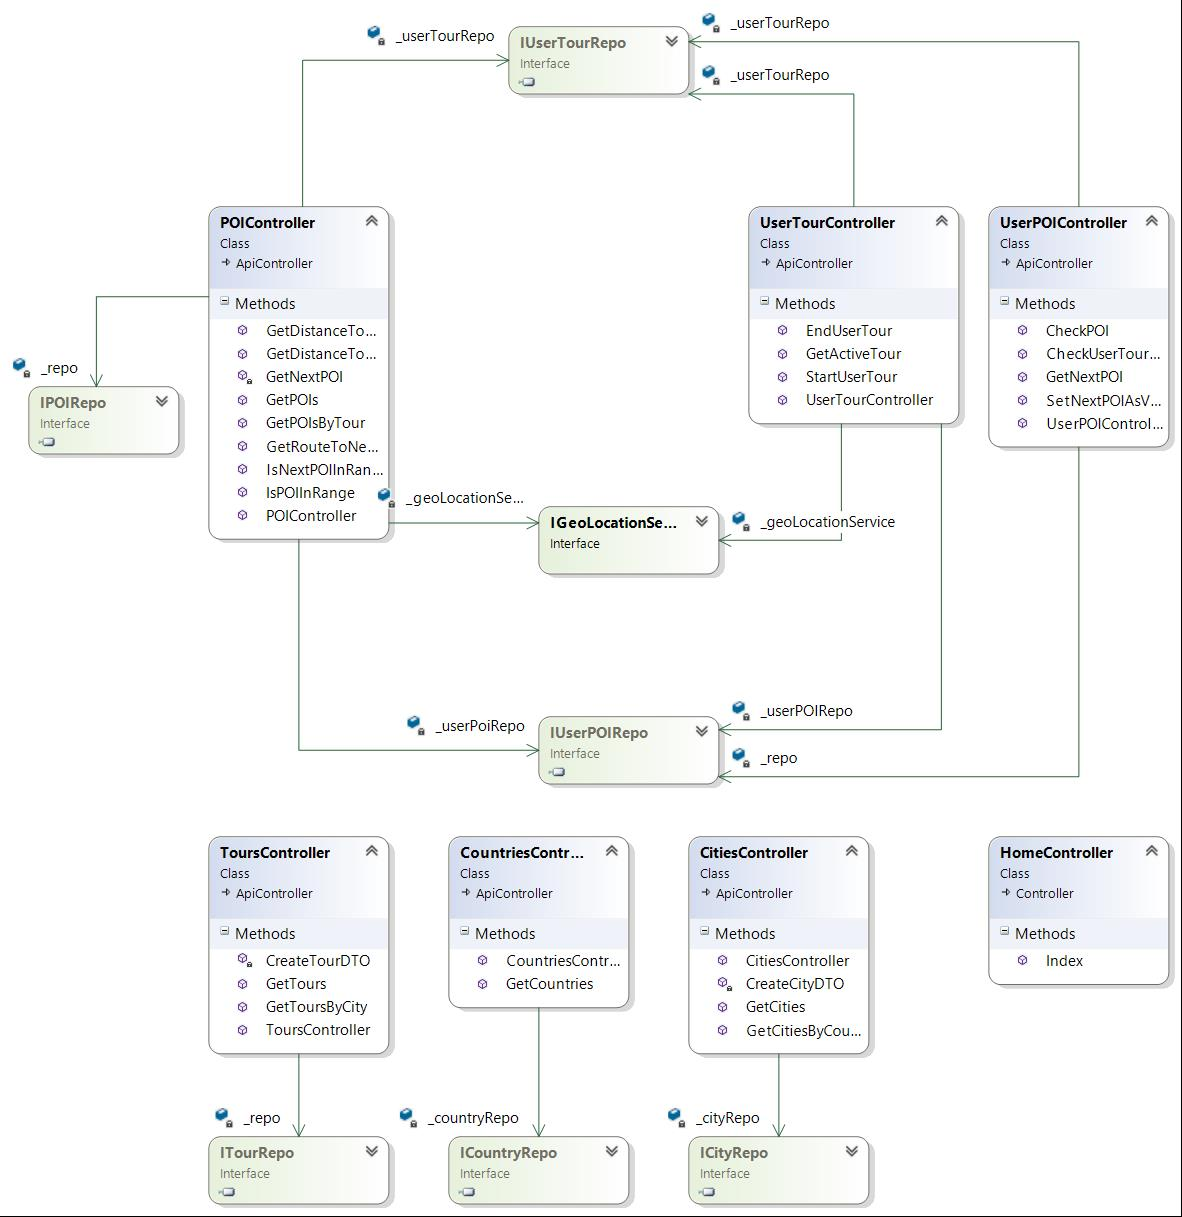
\includegraphics{klassendiagramm_backend1}
  \caption{Klassendiagramm mit Zusammenspiel der Controller und den jeweiligen Repositories}
\end{figure}

Die Controller weisen die in der Service API beschriebenen Funktionalit\"aten und Verantwortlichkeiten auf. Sie
behandeln alle ankommenden Requests und verwenden daf\"ur 1-n Repositories (da es sich nicht um reine CRUD Controller
handelt, k\"onnen auch mehrere Repositories verwendet werden) um die Daten aus der Datenbank zu holen und beliebige
Services, wie zum Beispiel den GeoLocationService, welcher einen Wrapper f\"ur die Google Maps Geo Location Services
implementiert. Services und Repositories werden wie bereits beschrieben \"uber Dependency Injection den Controllern zur
Verf\"ugung gestellt. Der HomeController dient als Einstiegspunkt der WebApplikation und ist daher kein API Controller.
Er liefert eine HTML View zur\"uck.

Die DTO Klassen sind erweiterte Datenklassen basierend (aber nicht vererbt) auf den vom Entity-Framework automatisch
generierten Datenklassen. Dies erm\"oglicht eine Erg\"anzung der Attribute um aggregierte oder separierte Werte.

\begin{figure}
  \centering
  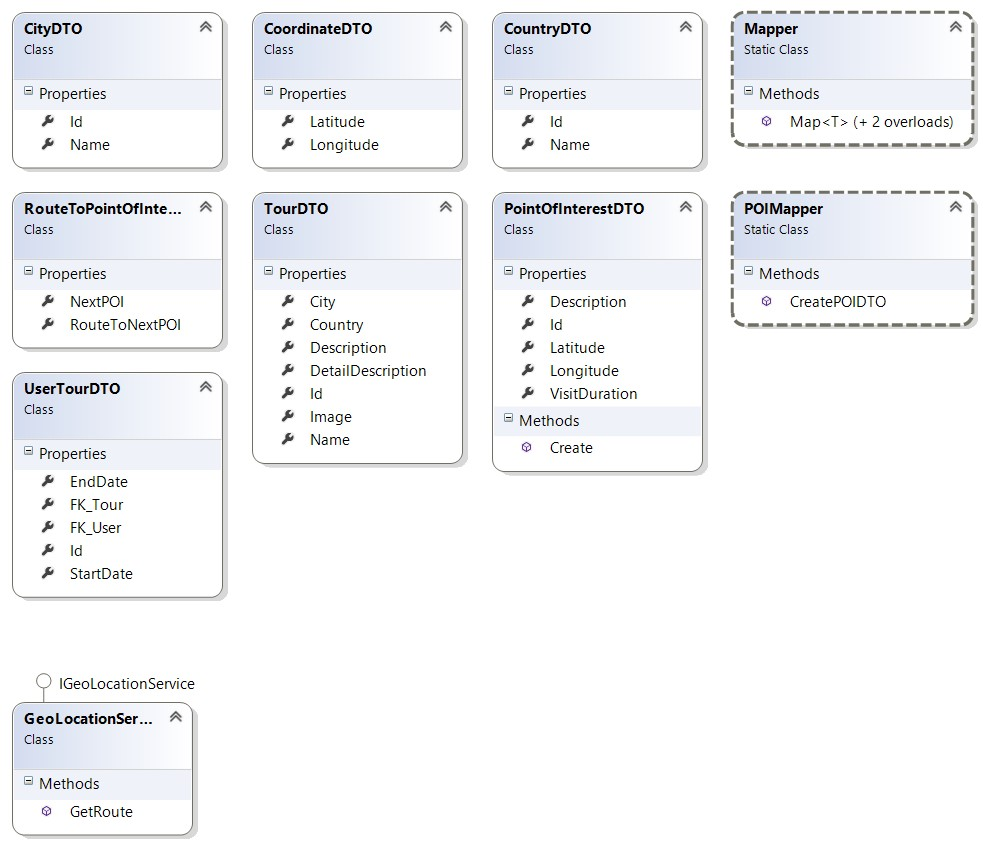
\includegraphics{klassendiagramm_backend2}
  \caption{Klassendiagramm DTO Klassen}
\end{figure}

Hier speziell zu erw\"ahnen sind die statische Mapper Klasse und der wiederverwendbare POIMapper. Die generische Mapper
Klasse mappt mit Hilfe von Reflection eine Datenklasse des Entity-Frameworks direkt auf gleichnamige Felder der
gew\"unschten DTO Klasse. Diese Funktionalit\"at kann f\"ur alle Felder verwendet werden die eins zu eins in beiden
Datenklassen vorhanden sind und den gleichen Datentypen besitzen. Ein manuelles Mappen dieser Felder ist damit nicht
mehr notwendig. Der POIMapper stellt die manuelle Mapping-Logik z.B. f\"ur das Aufsplitten der Geo-Koordinaten in
Latitude und Longitude in wiederverwendbarer Form bereit. Er liefert eine LINQ Function-Expression zur\"uck, welche die
Mapping-Logik definiert.

Die Repository Klassen implementieren das jeweilige von den Controllern von aussen her verwendete Interface.

\begin{figure}
  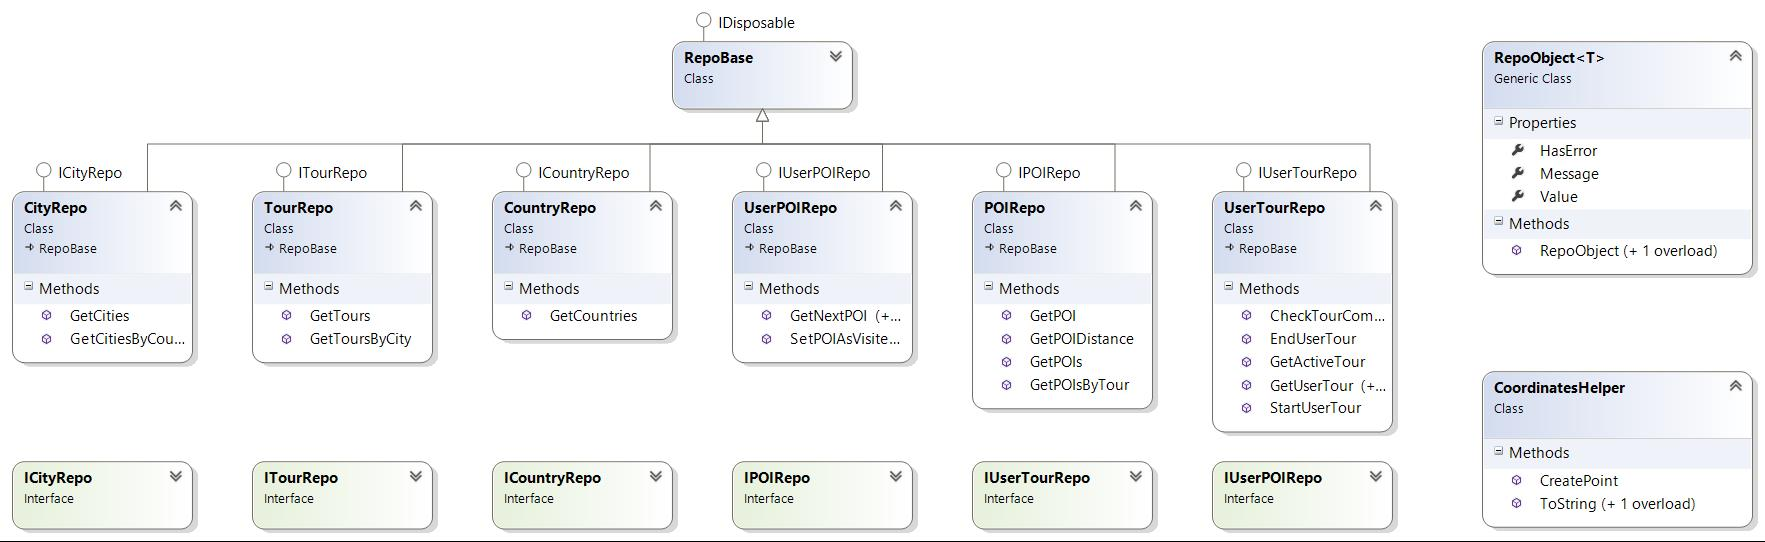
\includegraphics{klassendiagramm_backend3}
  \caption{Klassendiagramm der Repository Klassen}
\end{figure}

Die einzelnen Repositories implementieren den Zugriff \"uber LINQ-Queries auf die vom Vorbild der Datenbank generierten
Datenklassen\--Objekte. Sie sind alle von der Klasse RepoBase abgeleitet. RepoBase \"offnet bei der Instanzierung
automatisch eine Datenbankverbindung und stellt diese Verbindung den abgeleiteten Klassen zur Verf\"ugung. Die fachlichen und
funktionalen Verantwortlichkeiten werden analog zu den Zust\"andigkeiten der Controller implementiert. Im Kapitel
Service API werden daf\"ur die notwendigen Begriffe und Unterteilungen detailliert erl\"autert.

Speziell sind hier die Klassen RepoObject und CoordinatesHelper. Das RepoObject soll als R\"uckgabewert aller
Repo-Methoden dienen. Es beinhaltet ein Feld f\"ur den Wert als generisches IQueryable, ein Feld f\"ur eine Fehler-
oder Info-Message und ein Flag, ob ein Fehler aufgetreten ist. Mit dieser Struktur kann eine nicht sehr effiziente
Try-Catch-Throw Methodik vermieden und eine R\"uckgabe als weiterverwendbares IQueryable erzwungen werden.

Der CoordinatesHelper \"ubersetzt das MSSQL Datenbankformat der Geo-Koordinaten in einzelne ben\"otigte Werte wie
L\"angen- und Breitengrad und umgekehrt.

\subsection{Entity Relationship Diagram}\label{erm}
Als Erg\"anzung und zum besseren Verst\"andnis der Zusammenh\"ange nachfolgend das Diagramm des Datenbankmodels.

\begin{figure}
  \centering
  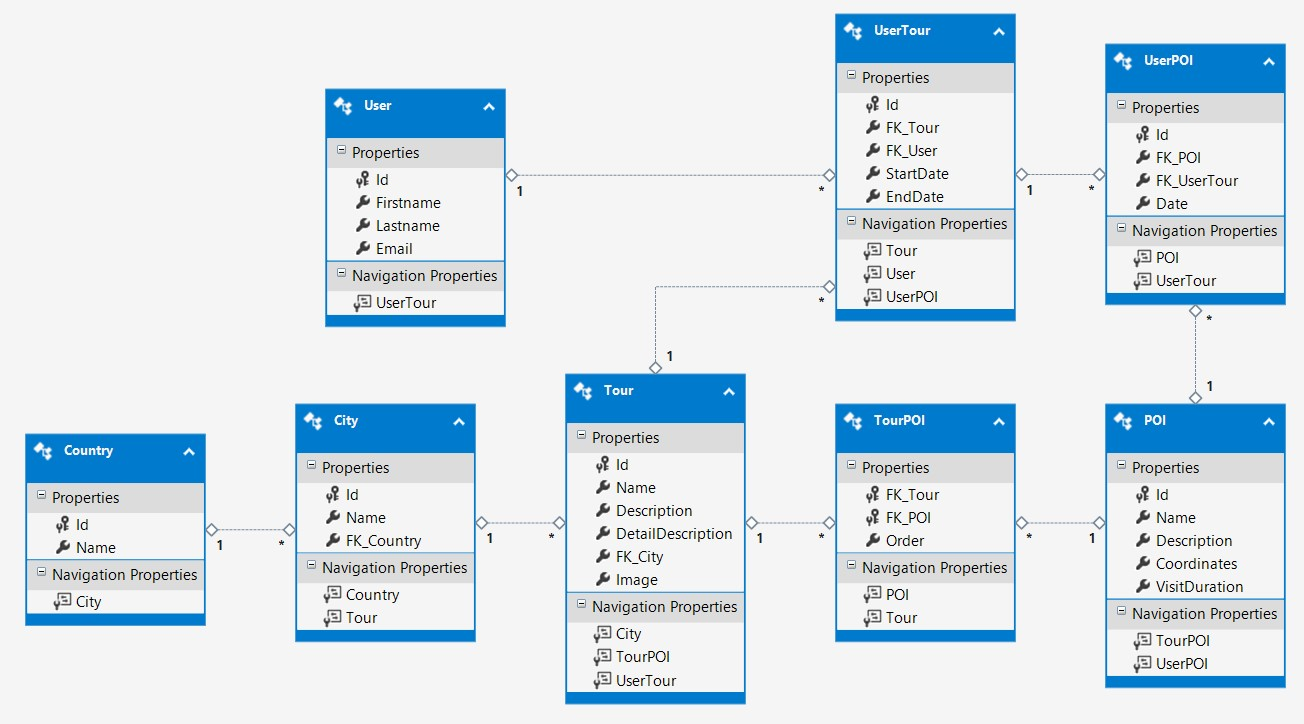
\includegraphics{erm}
  \caption{Entity Relationship Diagram}
\end{figure}

\section{Interaktionsdiagramme}\label{interaktionsdiagramme}
Im folgenden Kapitel zeigen wir die wichtigsten Interaktionsdiagramme unseres Backend und der Frontend-Applikation auf.

\subsection{Backend}\label{backend}

\subsubsection{Tour starten}
Bei dem Prozess ``Tour starten'' im Backend werden zuerst der mitgegebenen Benutzerdaten
überprüft und der Benutzer aus der Datenbank geladen. Anschliessend wird die angeforderte
Tour aus der Datenbank geladen und die Tour ``gestartet'' falls diese nicht schon gestartet ist.

\begin{figure}
  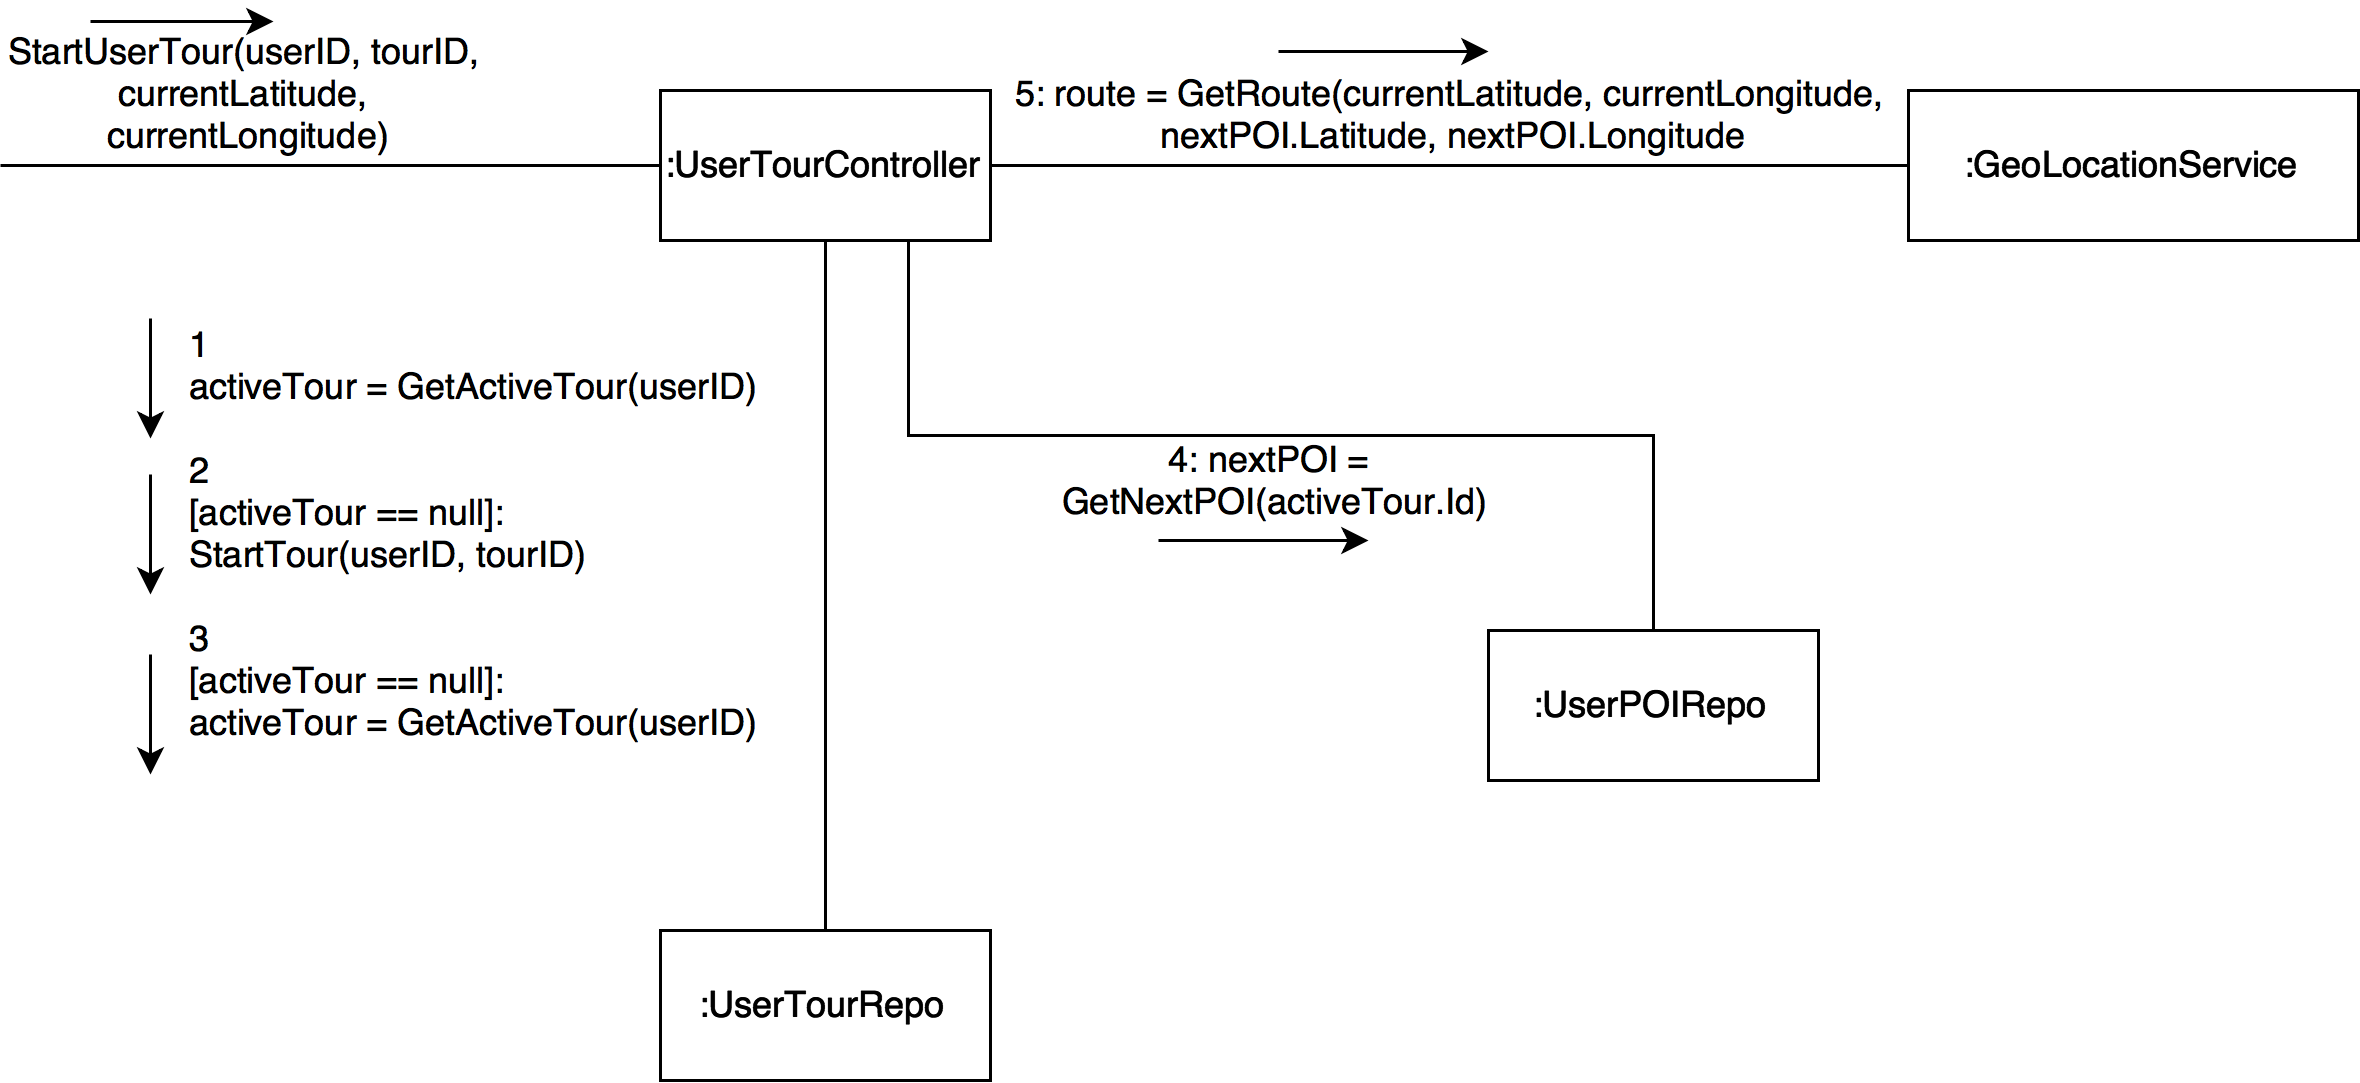
\includegraphics{Kommunikationsdiagramm_StartTour}
  \caption{Kommunikationsdiagramm Tour starten}
\end{figure}

\subsubsection{Route zu POI}
Im Ablauf ``Route zu POI'' werden zuerst die Benutzerdaten überprüft und der Benutzer aus
der Datenbank geladen. Anschliessend wird der vom Benutzer der Frontend-Applikation angestrebte
POI aus der Datenbank geladen und aufgrund der aktuellen Position die Route zum angestrebten
POI mittels Google Maps API berechnet und zurück gegeben.

\begin{figure}
  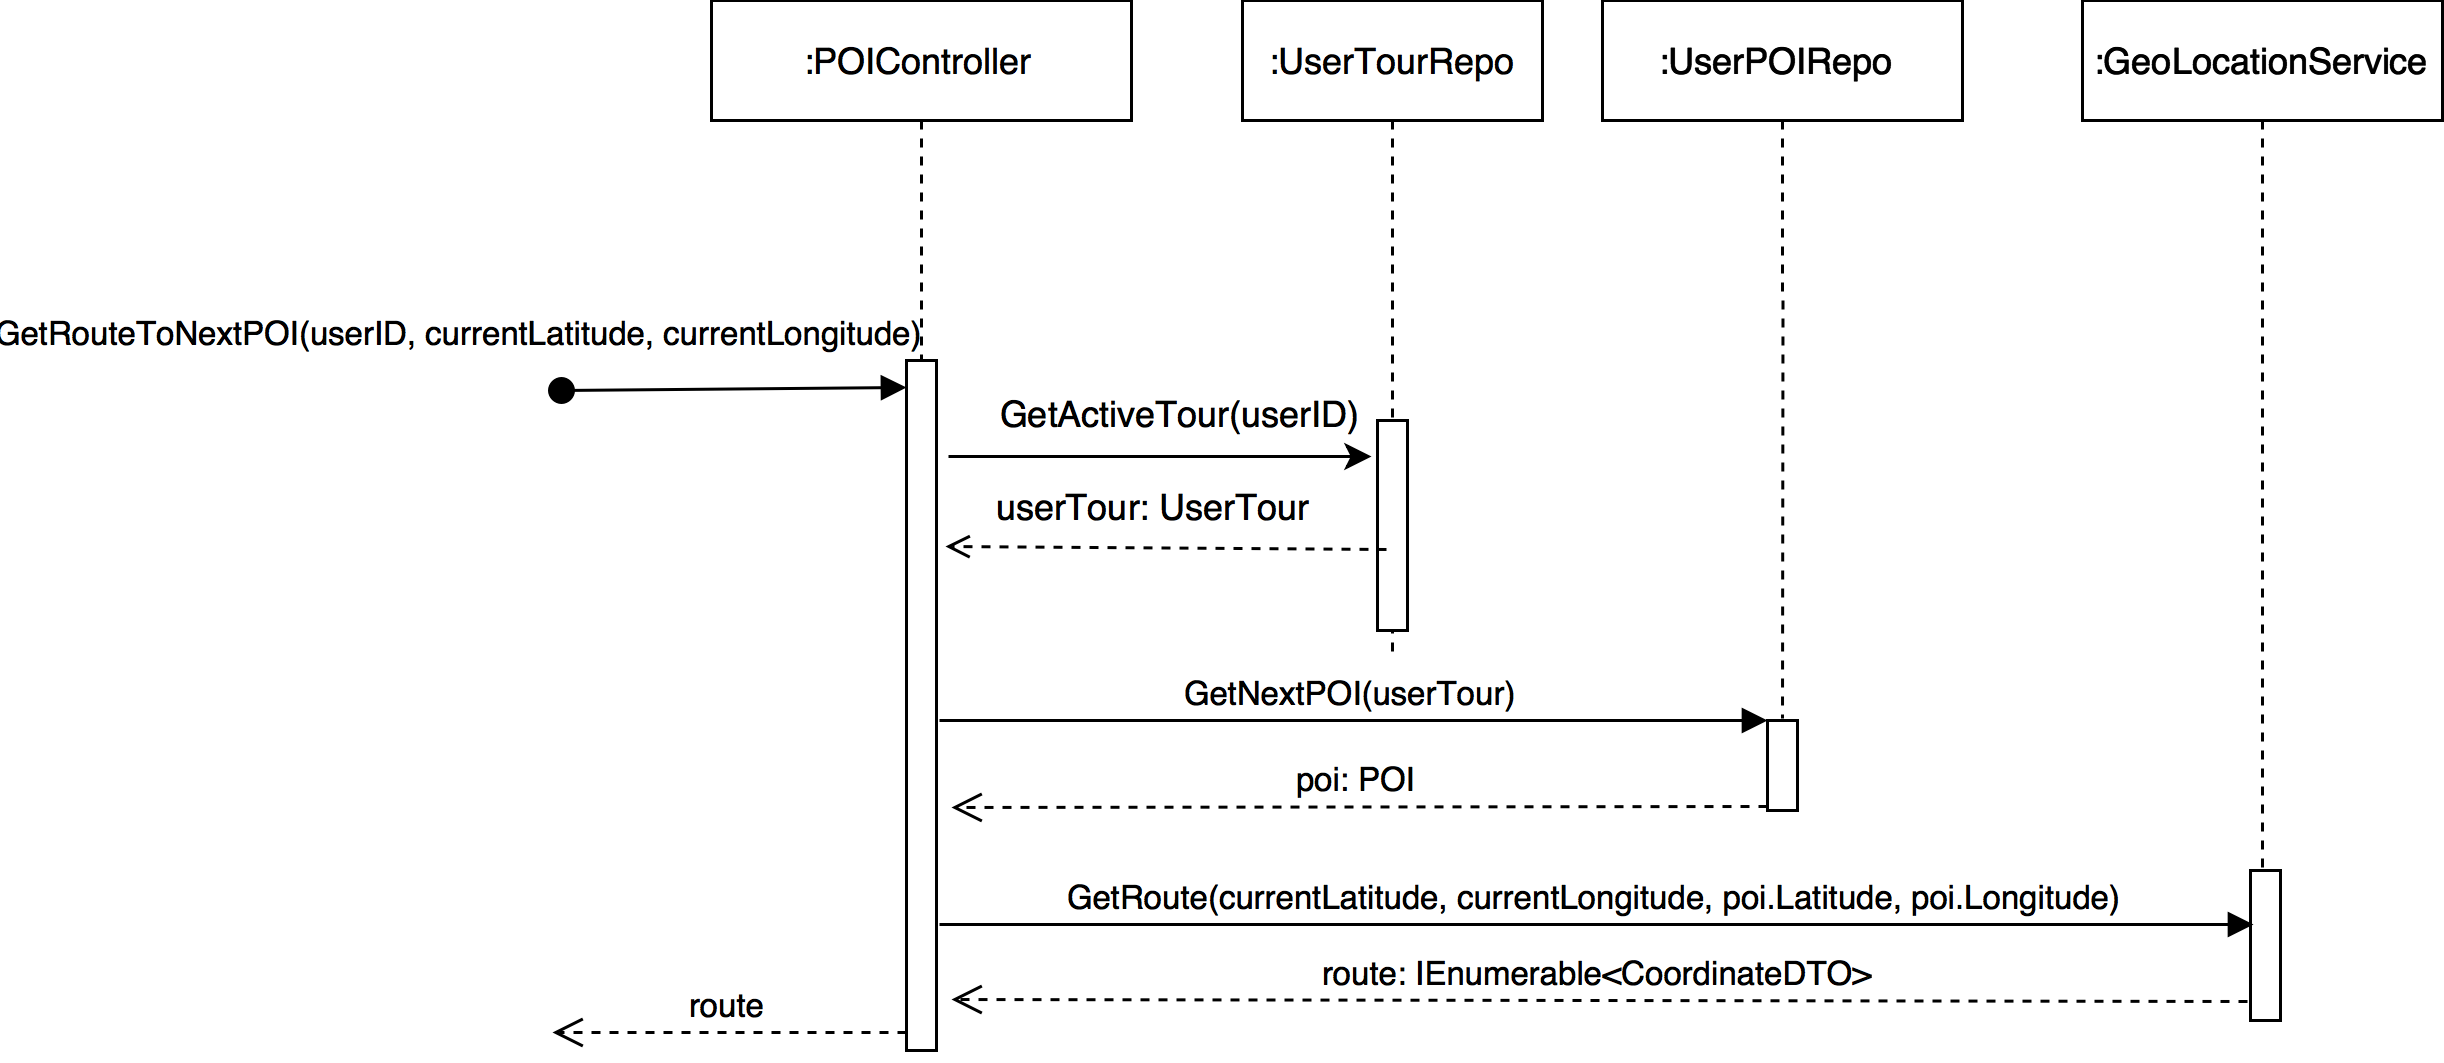
\includegraphics{Sequenzdiagramm_GetRouteToPoi}
  \caption{Sequenzdiagramm Route zu POI}
\end{figure}

\subsection{Frontend}\label{frontend}
\subsubsection{Tour Liste anzeigen}\label{frontend-listactivity}
Dieser Ablauf zeigt den Prozess wie die Liste der verfügbaren Touren in der Applikation
angezeigt wird. Über den \textbf{RequestQueuer} werden asynchron die Touren vom Backend geladen.
Der \textbf{RequestQueuer} führt bei erfolgreicher Serverantwort das Callback aus, welches
wiederum die Touren in der View setzt und diese aktualisiert.

\begin{figure}
  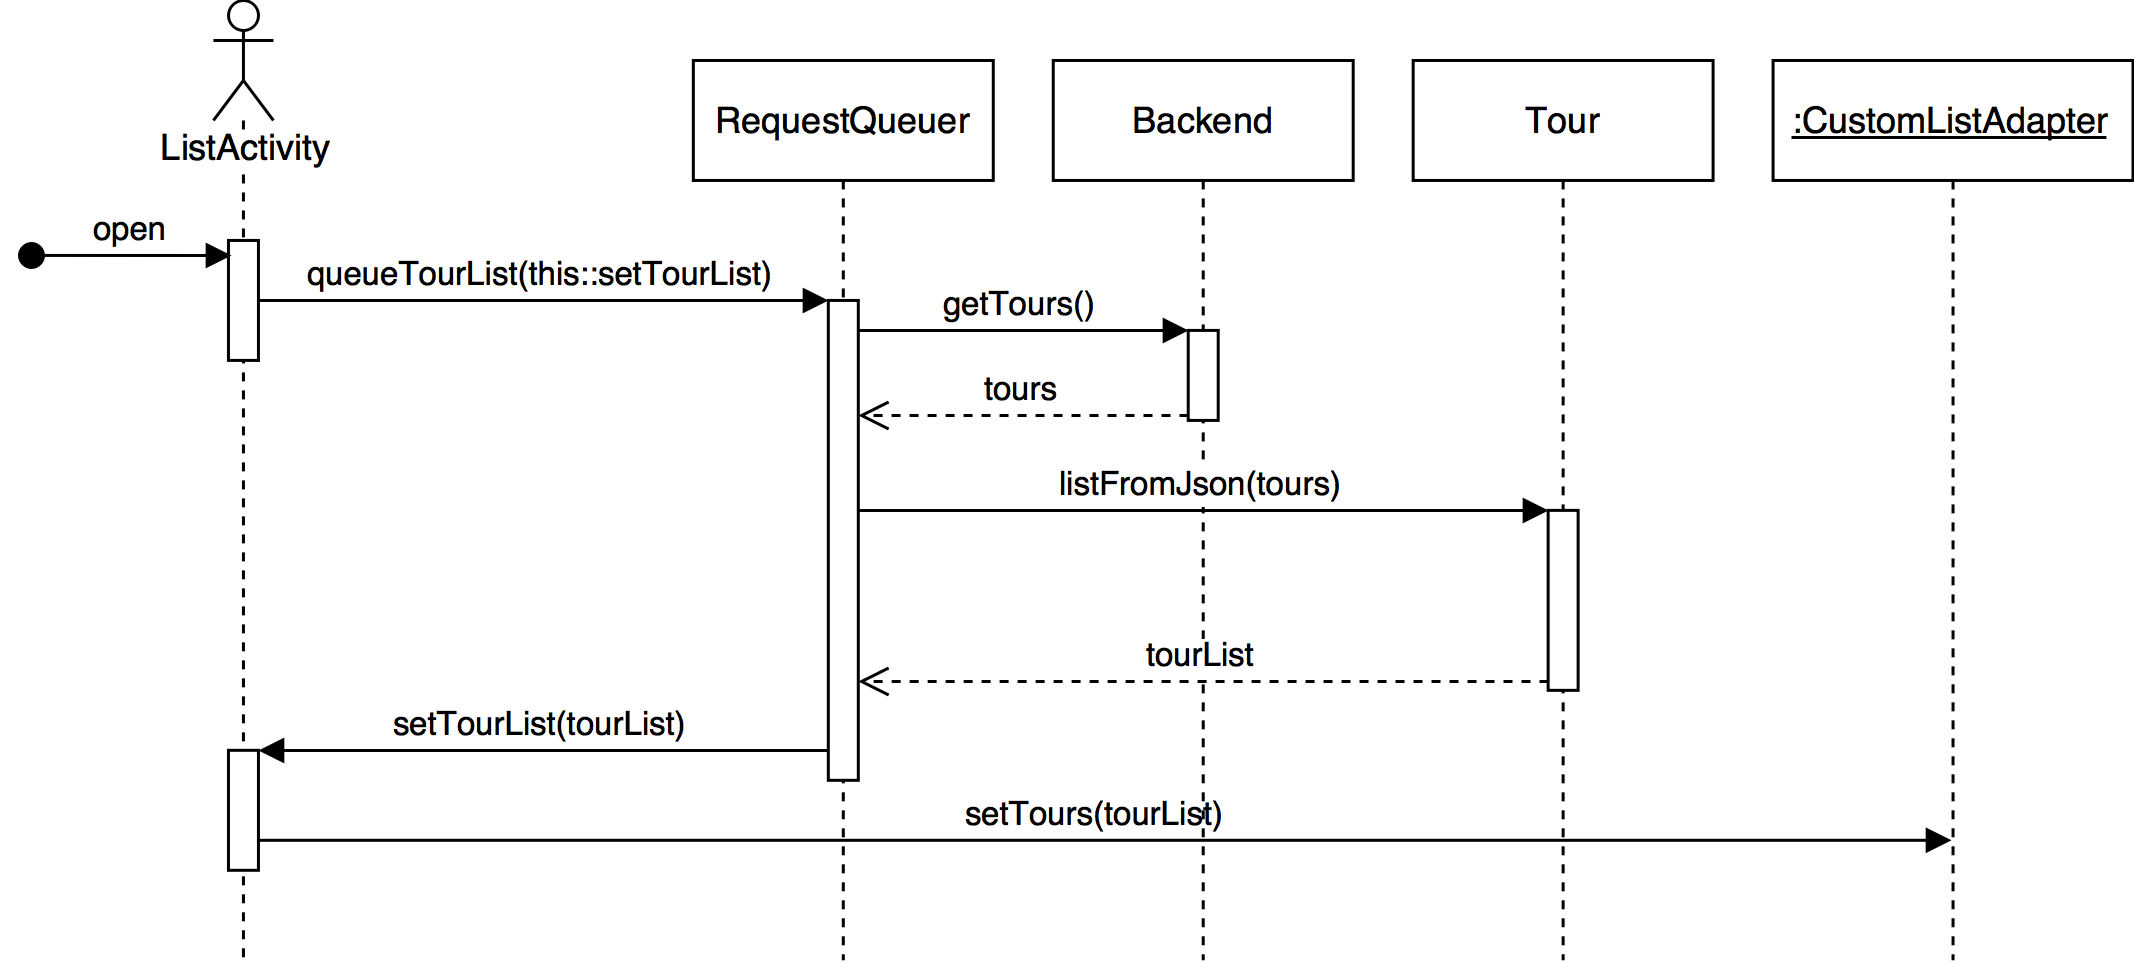
\includegraphics{Sequenzdiagramm_ListActivity}
  \caption{Sequenzdiagramm Tour Liste anzeigen}
\end{figure}

\subsubsection{Tour Details anzeigen}
Dieser Vorgang funktioniert ähnlich wie \fullref{frontend-listactivity}. Mittels
\textbf{RequestQueuer} werden alle POIs der ausgewählten Tour - welche der Activity übergeben
wurde - geladen, ebenfalls mittels Callback. Anschliessend werden die Daten der View
übergeben und die Karte gezeichnet.

\begin{figure}
  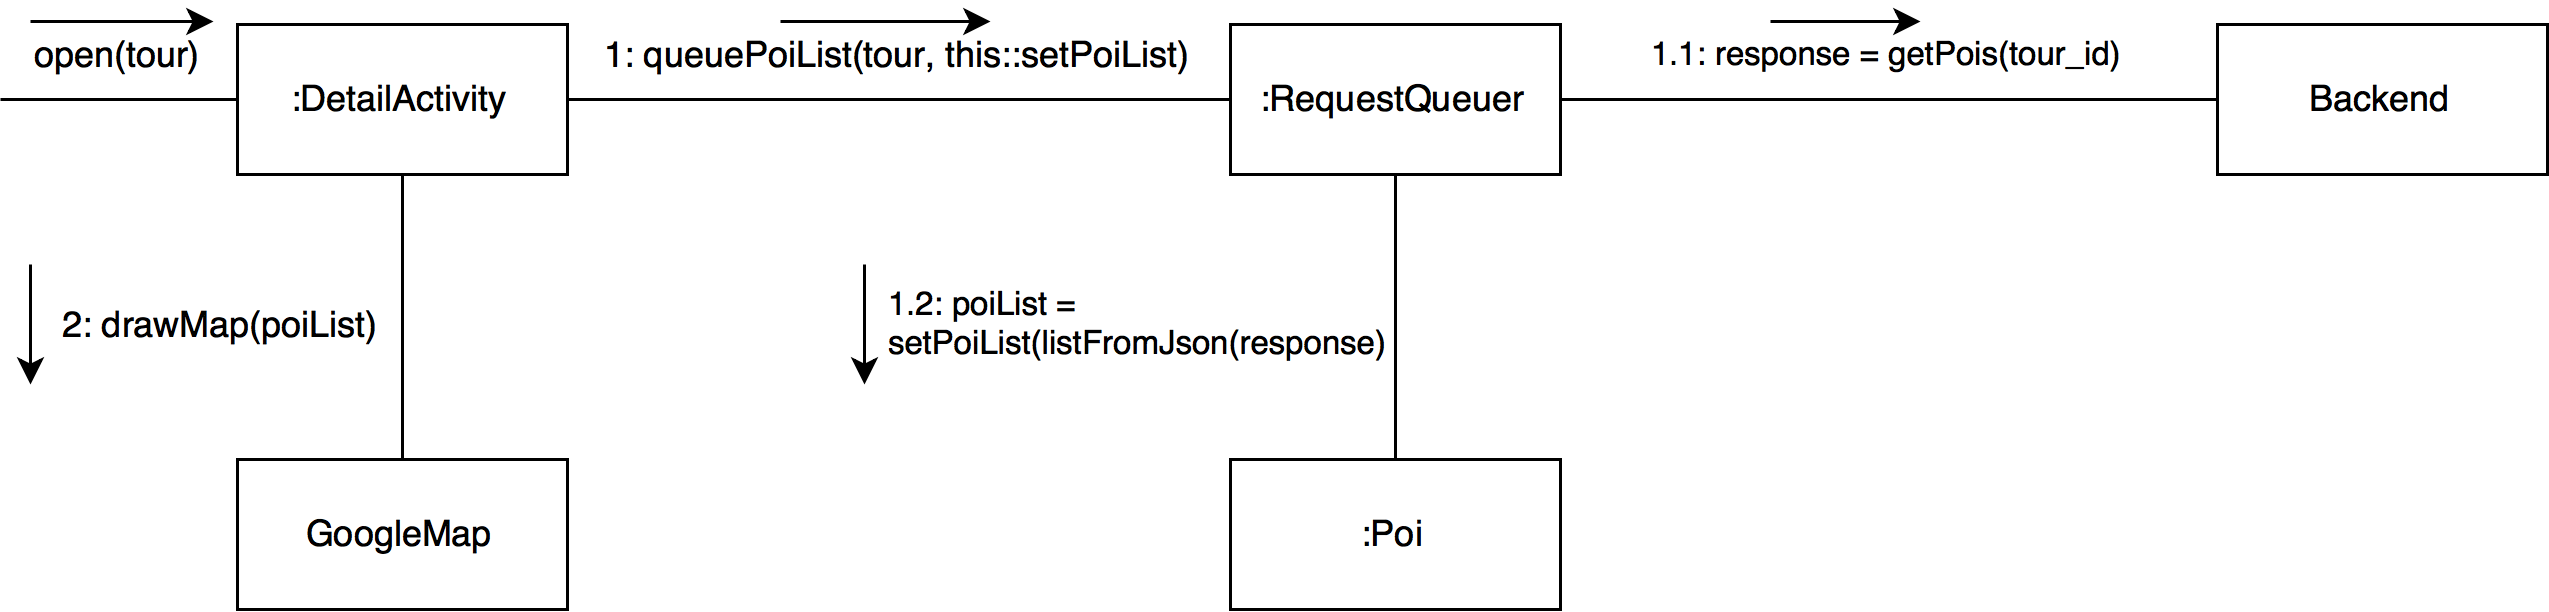
\includegraphics{Kommunikationsdiagramm_DetailActivity}
  \caption{Kommunikationsdiagramm Tour Details anzeigen}
\end{figure}

\subsubsection{Checke, ob bei POI angekommen}
Das Diagram zeigt den wiederkehrenden Prozess wobei überprüft wird, ob der Benutzer beim
ausgewählten POI angekommen ist. Der Google Maps Service ruft herzu bei der Veränderung
der Position eine Funktion auf. Diese benutzt den \textbf{RequestQueuer} um die Position
auf dem Backend zu überprüfen.

\begin{figure}
  \includegraphics{Sequenzdiagramm_IsNearPoi}
  \caption{Sequenzdiagramm Check ob bei POI angekommen}
\end{figure}

\subsubsection{Foto aufnehmen}
Mit dem Ablauf ``Foto aufnehmen'' wird aufgezeigt wie ein Foto mit der Gerätekamera
aufgenommen wird und diese Anschliessend zur Tour abgelegt wird.

\begin{figure}
  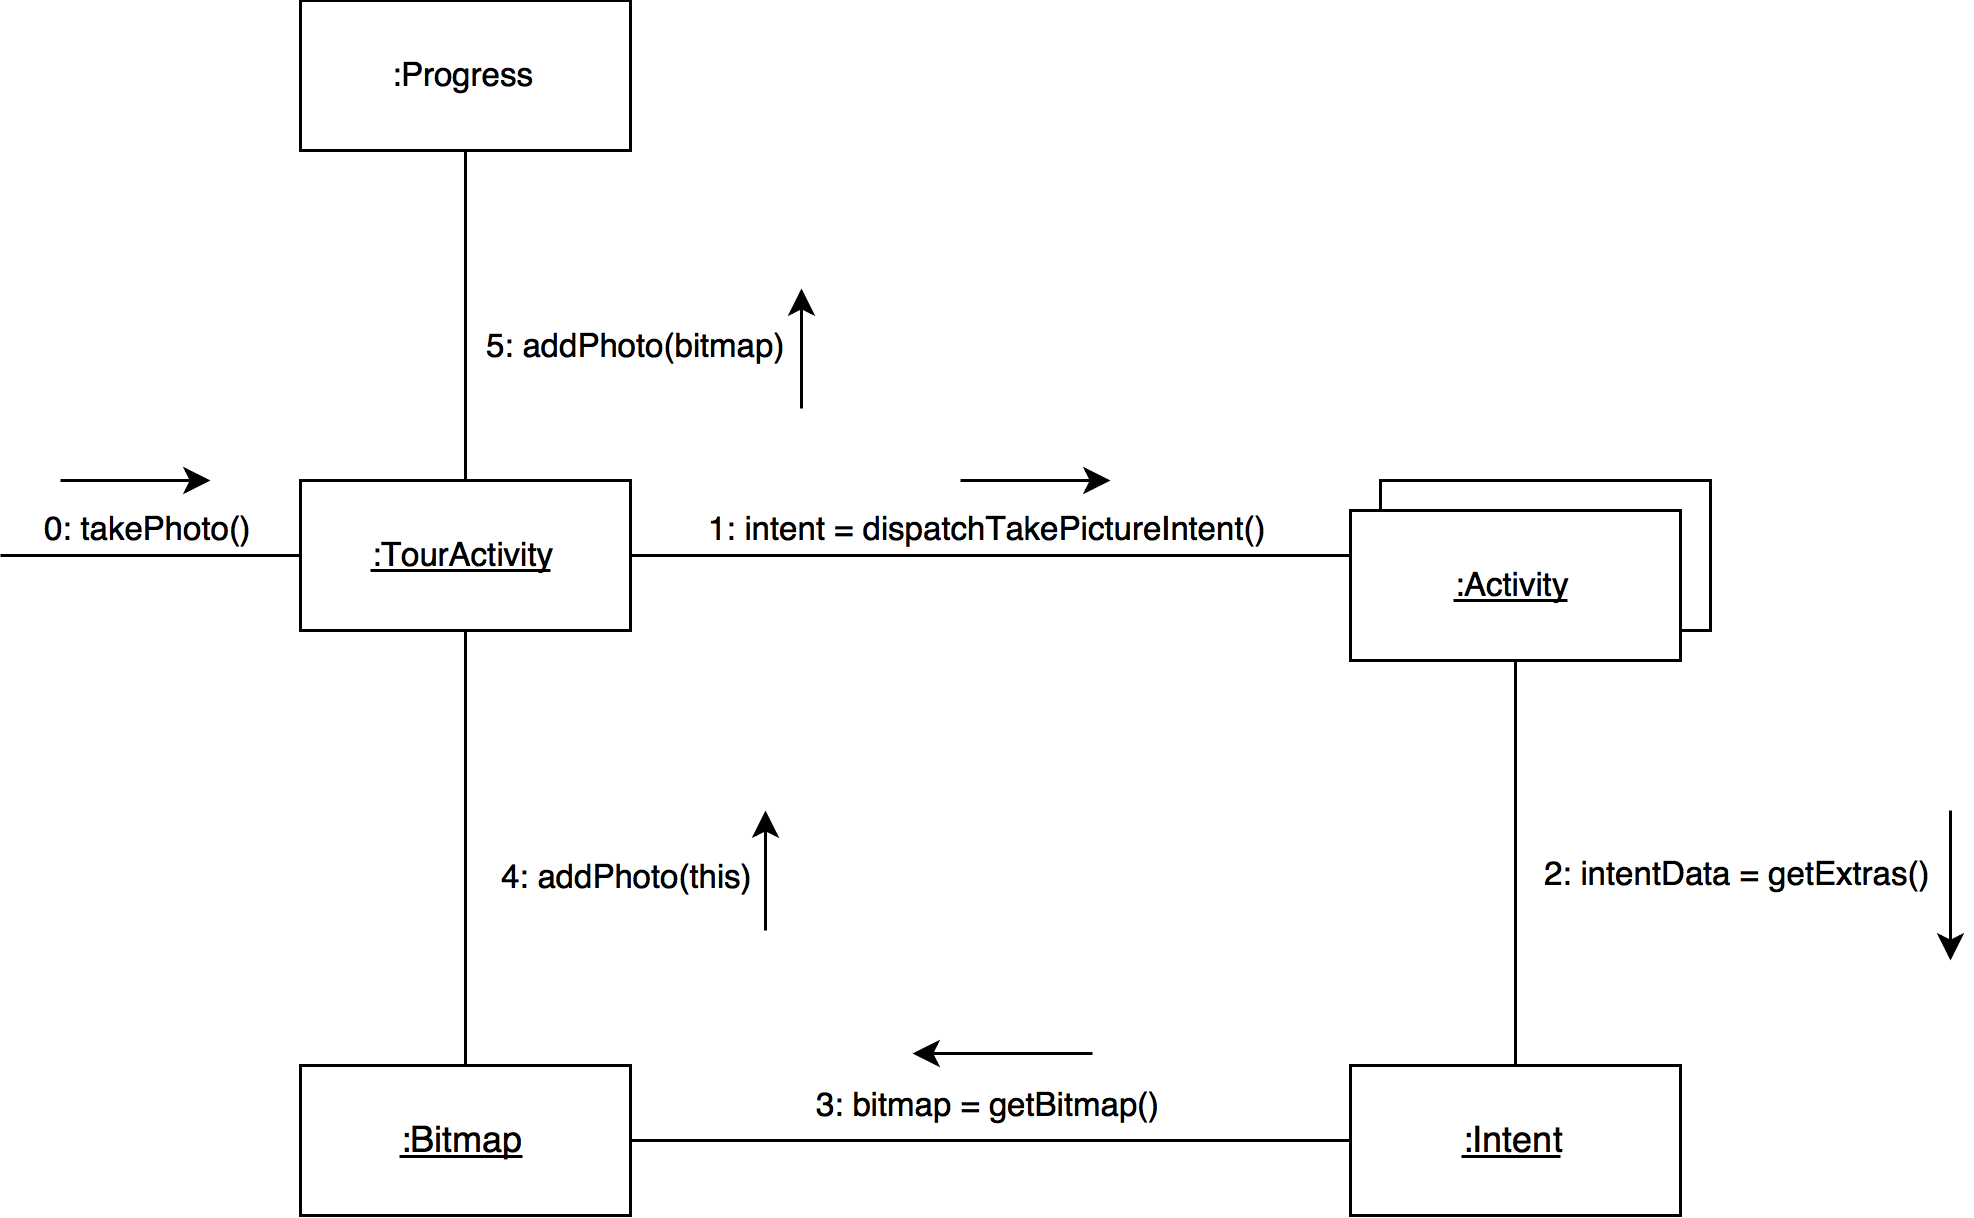
\includegraphics{Kommunikationsdiagramm_TakePhoto}
  \caption{Kommunikationsdiagramm Foto aufnehmen}
\end{figure}

\subsubsection{Summary anzeigen}
Dieser Vorgang zeigt den Abschluss einer Tour auf, wobei eine Übersicht der Tourdaten
generiert und angezeigt wird.
\begin{figure}
  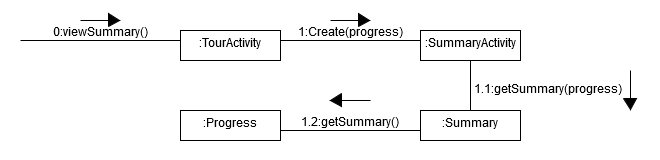
\includegraphics{Kommunikationsdiagramm_SummaryActivity}
  \caption{Kommunikationsdiagram Summary anzeigen}
\end{figure}

\newpage
\section{GUI-Design}\label{gui-design}
Die App startet auf der Anzeige ``ListActivity'' auf welchem alle verfügbaren Touren angezeigt
werden. Mit einem Klick auf eine Tour wird die Anzeige ``DetailActivity'' geöffnet und eine
Übersicht über die gewählte Tour wird sichtbar.

\begin{figure}
  \centering
  \begin{minipage}[b]{0.48\textwidth}
    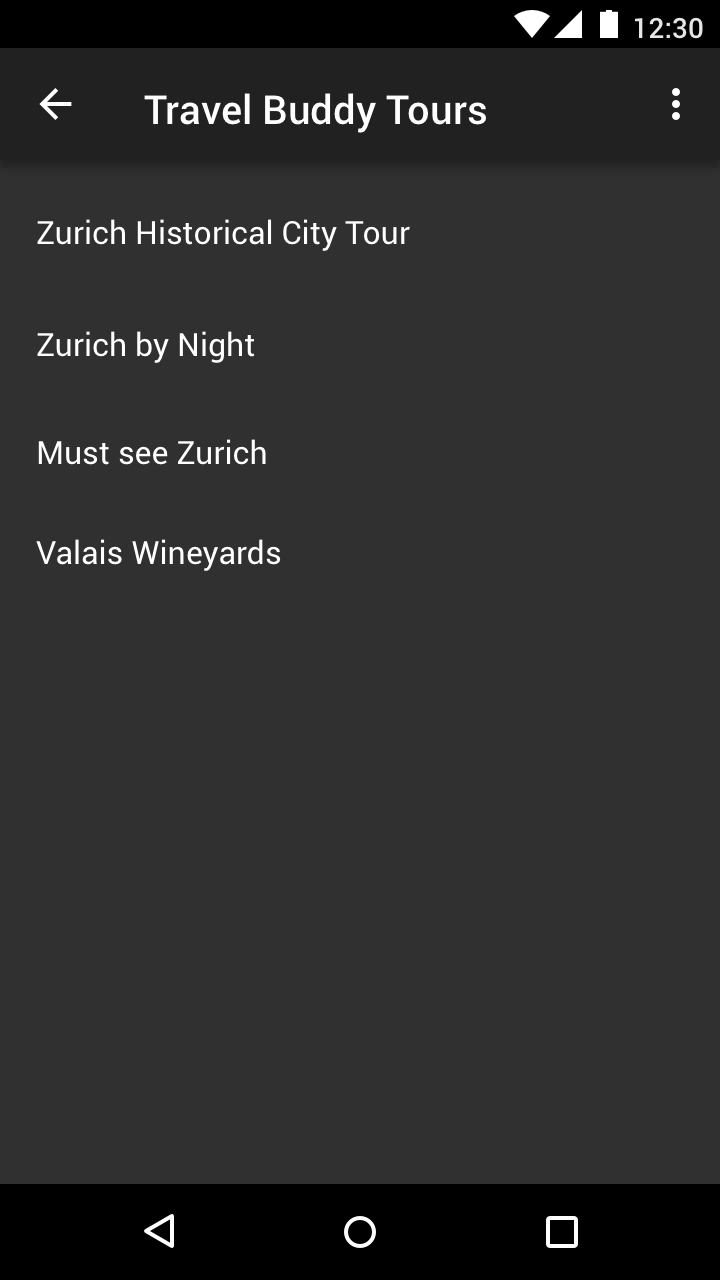
\includegraphics[width=\textwidth]{ListActivity}
    \caption{Anzeige ListActivity}
  \end{minipage}
  \hfill
  \begin{minipage}[b]{0.48\textwidth}
    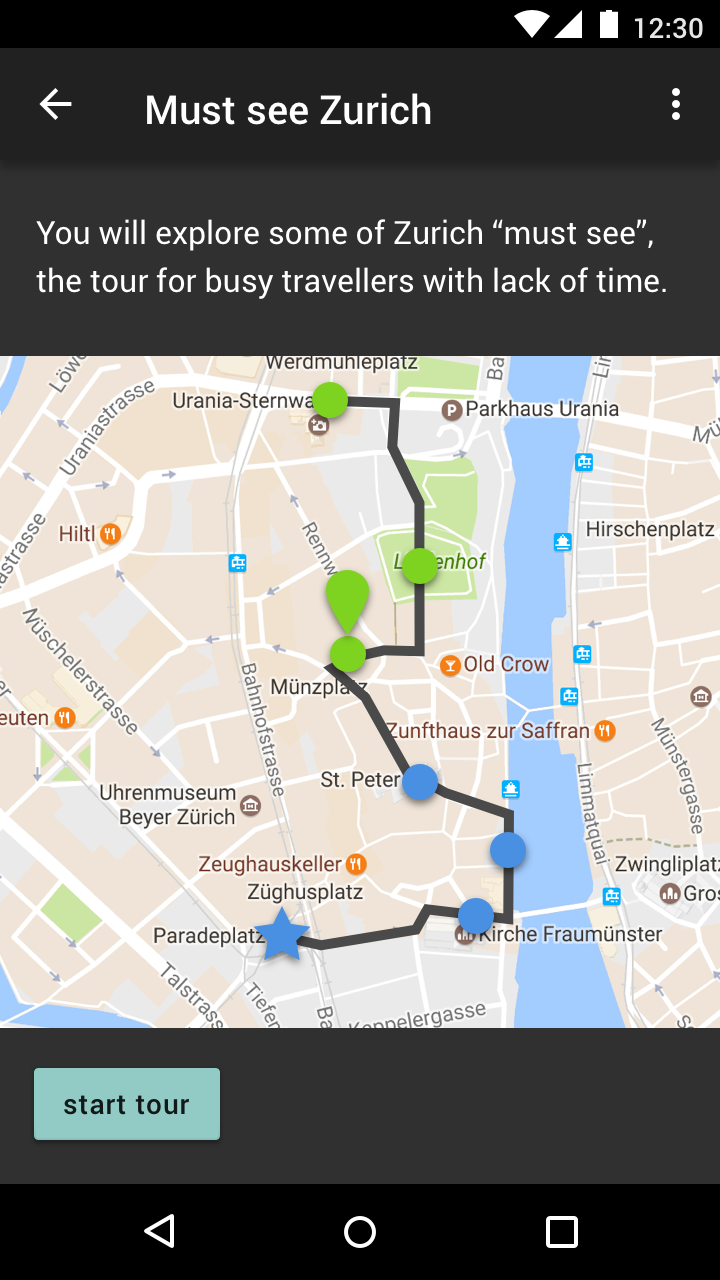
\includegraphics[width=\textwidth]{DetailActivity}
    \caption{Anzeige DetailActivity}
  \end{minipage}
\end{figure}

\newpage
Über den Button ``Tour starten'' gelangt
man weiter zur Ansicht ``TourActivity'' worauf jeweils der Weg zum nächsten POI ersichtlich ist.
Abgeschossen wird eine Tour mit der Anzeige ``SummaryActivity''.

\begin{figure}
  \centering
  \begin{minipage}[b]{0.48\textwidth}
    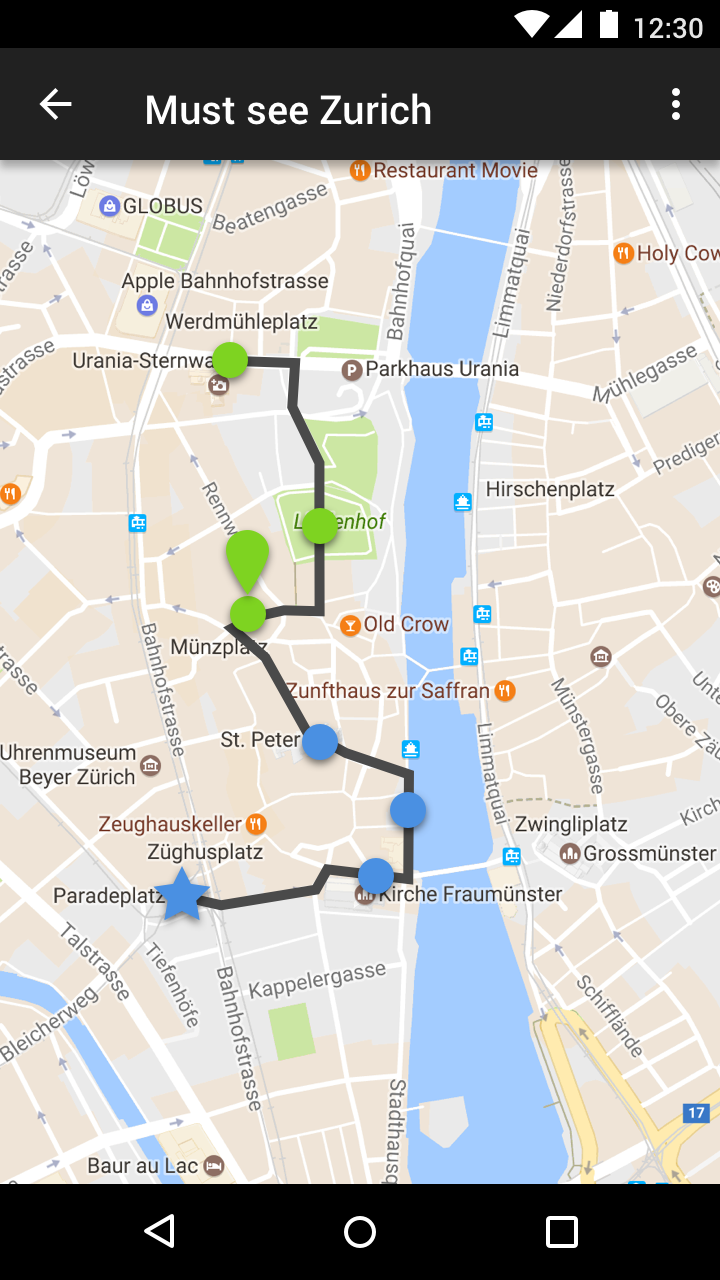
\includegraphics[width=\textwidth]{TourActivity}
    \caption{Anzeige TourActivity}
  \end{minipage}
  \hfill
  \begin{minipage}[b]{0.48\textwidth}
    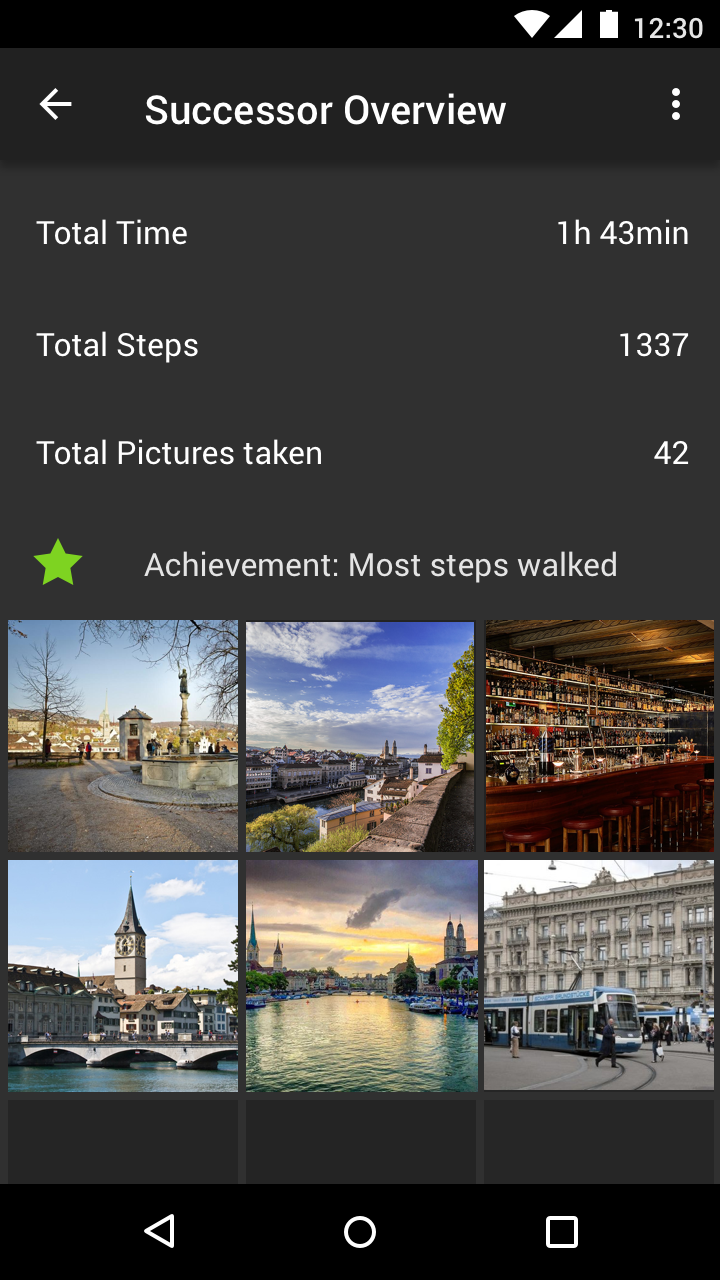
\includegraphics[width=\textwidth]{SummaryActivity}
    \caption{Anzeige SummaryActivity}
  \end{minipage}
\end{figure}

\newpage
\section{Glossar}\label{glossar}
\begin{longtabu} to \textwidth { | l | X[l] | }
\hline
\textbf{Begriff} & \textbf{Bemerkung}\\\hline
\endhead

Agency/Agencies & Engl. Agenturen\\\hline
Smartphone & Mobilgerät mit erweiterten Funktionen\\\hline
Android & Betriebssystem für Mobilgeräte\\\hline
Mobile Application/Mobile App & Mobile Applikation, Synonym für mobile Applikation auf Smartphone\\\hline
Backend & Serverseitige Anwendung, stellt API zur Verfügung\\\hline
External Services & Engl. Externe Dienste, Dienste die nicht vom Programm selber ausgeführt werden, wie z.B. Location Services\\\hline
Fallback & Ausweichlösung/Alternativlösung\\\hline
Frontend & Benutzerseitige Anwendung, hier App welche API konsumiert\\\hline
GPS & Global Positioning System, globales Satelliten Navigationsnetz\\\hline
Marker & Symbol, welches einen Punkt auf der Karte markiert\\\hline
Natives Features & Funktionen, die ein Gerät ohne weitere Software besitzt\\\hline
ÖV & Abkz. Öffentlicher Verkehr\\\hline
Point of Interest, POI & Engl. Ort von besonderem Interesse, bspw. Wahrzeichen\\\hline
Stakeholders & Engl. Interessenten\\\hline
Tech Stack & Eingesetzte Technologien\\\hline
Mockdaten & Daten mit gleicher Struktur wie echte Daten. Dient der lokalen Entwicklung, Testdaten \\\hline
Trip & Engl. Reise, enthält mehrere Touren\\\hline
Touristin & Die eigentliche Benutzerin der App\\\hline
POJO & Plain old Java object (Datenobjekt)\\\hline
PubSub & Publisher subscriber Pattern\\\hline
Singleton & Eine Klasse, von der nur eine Instanz erstellt werden kann.\\\hline
Intent & Intent bezeichnet hier eine Nachricht in Android. Der Name impliziert, dass Komponenten selber entscheiden ob sie auf diese Nachrichten reagieren oder nicht.\\\hline
\end{longtabu}


\section{Literatur}\label{literatur}
\begingroup
\renewcommand{\section}[2]{}%
  \begin{thebibliography}{9}
    \bibitem{TCA} URL: https://8thlight.com/blog/uncle-bob/2012/08/13/the-clean-architecture.html [Stand: 20.4.2017]
    \bibitem{CC} URL: http://blog.cleancoder.com/ [Stand: 20.4.2017]
    \bibitem{RV} URL: http://robovm.mobidevelop.com/ [Stand: 20.4.2017]
    \bibitem{MOE} URL: https://software.intel.com/en-us/multi-os-engine [Stand: 17.4.2017]
  \end{thebibliography}
\endgroup

\section{Abbildungsverzeichnis}\label{abbildungsverzeichnis}
\begingroup
\renewcommand{\section}[2]{}%
\hypersetup{linkcolor=black}
\listoffigures
\endgroup

\end{document}
